

\setcounter{chapter}{5}

\chapter{群论的进一步专题}

\section{\(p\)-群、幂零群与可解群}

设 \(p\) 是素数，\(G\) 是 \(p^a n\) 阶有限群，其中 \(p\) 不整除 \(n\). 回忆（有限）\textbf{\(p\)-群}是阶为 \(p\) 的幂的群。西罗定理表明 \(p\)-群作为 \(G\) 的子群大量存在，为了利用这一现象揭示有限群的结构，有必要建立 \(p\)-群的一些基本性质。下一节我们将把这些结果应用到许多具体情况中。

在给出关于 \(p\)-群的结果之前，我们首先回忆一个在前面习题中出现过的定义。

\begin{definition}
群 \(G\) 的\textbf{极大子群}是 \(G\) 的真子群 \(M\)，使得不存在满足 \(M < H < G\) 的 \(G\) 的子群 \(H\).
\end{definition}

由阶的考虑，有限群的每个真子群都包含在某个极大子群中。相反，无限群可能有也可能没有极大子群。例如，\(p\mathbb{Z}\) 是 \(\mathbb{Z}\) 的极大子群，而 \(\mathbb{Q}\)（加法下）没有极大子群（参见本节末习题 16）。

我们现在把所需的 \(p\)-群的全部性质收集到一个综合定理中：

\begin{theorem}\label{thm:6.1}
设 \(p\) 是素数，\(P\) 是 \(p^a\) 阶群（\(a \geq 1\)）。则

\begin{enumerate}[label=(\arabic*)]
\item \(P\) 的中心非平凡：\(Z(P) \neq 1\).
\item 若 \(H\) 是 \(P\) 的非平凡正规子群，则 \(H\) 与中心的交非平凡：\(H \cap Z(P) \neq 1\). 特别地，每个 \(p\) 阶正规子群都包含在中心中。
\item 若 \(H\) 是 \(P\) 的正规子群，则对 \(|H|\) 的每个因子 \(p^b\)，\(H\) 含有一个在 \(P\) 中正规的 \(p^b\) 阶子群。特别地，对每个 \(b \in \{0, 1, \ldots, a\}\)，\(P\) 有 \(p^b\) 阶正规子群。
\item 若 \(H < P\)，则 \(H < N_P(H)\)（即 \(P\) 的每个真子群都是它在 \(P\) 中正规化子的真子群）。
\item \(P\) 的每个极大子群的指数为 \(p\)，且在 \(P\) 中正规。
\end{enumerate}
\end{theorem}

\begin{proof}
这些结果最终依赖于类方程，读者回顾 4.3 节可能会有帮助。

（1）是第 4 章定理 8，也是（2）在 \(H = P\) 时的特殊情形。因此我们首先证明（2）；我们不会引用第 4 章定理 8，尽管下面的论证只是第 4 章中那个论证的略微推广。设 \(H\) 是 \(P\) 的非平凡正规子群。回忆对 \(P\) 的每个共轭类 \(C\)，或者 \(C \subseteq H\)，或者 \(C \cap H = \varnothing\)，因为 \(H\) 正规（这个容易的事实已在定理 4.12 前的评注中证明）。取 \(P\) 的共轭类的代表元
\[
a_1, \ldots, a_k, a_{k+1}, \ldots, a_r,
\]
其中 \(a_1, \ldots, a_k \in H\)，\(a_{k+1}, \ldots, a_r \notin H\). 对所有权 \(i\)，设 \(C_i\) 是 \(a_i\) 在 \(P\) 中的共轭类。于是
\[
C_i \subseteq H\ (1 \leq i \leq k), \qquad C_i \cap H = \varnothing\ (k+1 \leq i \leq r).
\]
必要时重新给 \(a_1, \ldots, a_k\) 编号，可设 \(a_1, \ldots, a_s\) 代表大小为 1 的类（即在 \(P\) 的中心中），\(a_{s+1}, \ldots, a_k\) 代表大小大于 1 的类。由于 \(H\) 是这些类的无交并，我们有
\[
|H| = |H \cap Z(P)| + \sum_{i=s+1}^{k} \frac{|P|}{|C_P(a_i)|}.
\]
现在 \(p\) 整除 \(|H|\)，且 \(p\) 整除和式中的每一项 \(\frac{|P|}{|C_P(a_i)|}\)，故 \(p\) 整除它们的差 \(|H \cap Z(P)|\). 这证明 \(H \cap Z(P) \neq 1\). 若 \(|H| = p\)，则由于 \(H \cap Z(P) \neq 1\)，必有 \(H \leq Z(P)\). 这完成了（2）的证明。

接下来我们对 \(a\) 作归纳证明（3）。若 \(a \leq 1\) 或 \(H = 1\)，结果是平凡的。因此假设 \(a > 1\) 且 \(H \neq 1\). 由（2），\(H \cap Z(P) \neq 1\)，故由柯西定理 \(H \cap Z(P)\) 含有 \(p\) 阶（正规）子群 \(Z\). 用横线记号表示过渡到商群 \(P/Z\). 这个商的阶为 \(p^{a-1}\)，且 \(\bar{H} \trianglelefteq \bar{P}\). 由归纳假设，对每个使 \(p^b\) 整除 \(|H|\) 的非负整数 \(b\)，存在 \(\bar{H}\) 的 \(p^b\) 阶子群 \(\bar{K}\) 在 \(\bar{P}\) 中正规。若 \(K\) 是 \(\bar{K}\) 在 \(P\) 中的完全原像，则 \(|K| = p^{b+1}\). 用这个过程得到的所有 \(H\) 的子群连同单位子群一起，为 \(|H|\) 的每个因子提供一个在 \(P\) 中正规的 \(H\) 的子群。第 3 部分的第二个论断是 \(H = P\) 的特殊情形。这证明了第 3 部分。

我们也对 \(|P|\) 作归纳证明（4）。若 \(P\) 阿贝尔，则 \(P\) 的所有子群都正规，结果平凡。因此可设 \(|P| > p\)（事实上由推论 4.9 有 \(|P| > p^2\)）。设 \(H\) 是 \(P\) 的真子群。由于 \(Z(P)\) 的所有元素与 \(P\) 的所有元素交换，\(Z(P)\) 正规化 \(P\) 的每个子群。由（1）\(Z(P) \neq 1\). 若 \(Z(P)\) 不含于 \(H\)，则 \(H\) 真包含在 \(\langle H, Z(P) \rangle\) 中，而后一子群包含在 \(N_P(H)\) 中，故（4）成立。因此可设 \(Z(P) \leq H\). 用横线记号表示过渡到商群 \(P/Z(P)\). 由（1）\(\bar{P}\) 的阶小于 \(P\)，故由归纳假设 \(\bar{H}\) 真包含在 \(N_{\bar{P}}(\bar{H})\) 中。由格子同构定理直接可得 \(N_P(H)\) 是 \(N_{\bar{P}}(\bar{H})\) 在 \(P\) 中的完全原像，因此在这种情形我们也得到 \(H\) 真包含在它在 \(P\) 中的正规化子中。这完成了归纳。

为证明（5），设 \(M\) 是 \(P\) 的极大子群。按定义 \(M < P\)，故由（4）\(M < N_P(M)\). 由极大性的定义必有 \(N_P(M) = P\)，即 \(M \trianglelefteq P\). 格子同构定理表明由于 \(M\) 是极大子群，\(P/M\) 是没有非平凡真子群的 \(p\)-群。但由（3），\(P/M\) 有整除 \(|P/M|\) 的每个阶的子群。唯一可能是 \(|P/M| = p\). 这证明了（5）并完成定理的证明。
\end{proof}

\begin{definition}
（1）对任意（有限或无限）群 \(G\)，归纳定义如下子群：
\[
Z_0(G) = 1,
\]
且 \(Z_{i+1}(G)\) 是 \(G\) 的包含 \(Z_i(G)\) 的子群，满足
\[
Z_{i+1}(G)/Z_i(G) = Z(G/Z_i(G))
\]
（即 \(Z_{i+1}(G)\) 是 \(G/Z_i(G)\) 的中心在自然投影下的完全原像）。子群链
\[
1 = Z_0(G) \leq Z_1(G) \leq Z_2(G) \leq \cdots
\]
称为 \(G\) 的\textbf{上中心列}。（“上”这个词表明 \(Z_i(G) \leq Z_{i+1}(G)\).）

（2）群 \(G\) 称为\textbf{幂零的}，若对某个 \(c \in \mathbb{Z}\) 有 \(Z_c(G) = G\). 最小的这样的 \(c\) 称为 \(G\) 的\textbf{幂零类}。
\end{definition}

本节末的一个习题表明 \(Z_i(G)\) 对所有 \(i\) 都是 \(G\) 的特征（因而正规）子群。从现在起我们自由地使用这一事实。

\textbf{注：}

（1）若 \(G\) 阿贝尔，则 \(G\) 幂零（类为 1，只要 \(|G| > 1\)），因为此时 \(G = Z(G) = Z_1(G)\). 应当把幂零群看作在结构层次中位于阿贝尔群与可解群之间（回忆可解群在 3.4 节引入；我们将在本节末进一步讨论可解群）：
\[
\text{循环群} \subsetneq \text{阿贝尔群} \subsetneq \text{幂零群} \subsetneq \text{可解群} \subsetneq \text{所有群}
\]
（我们不久将验证上面所有包含都是真包含）。

（2）对任意有限群，由阶的考虑必有整数 \(n\) 使 \(Z_n(G) = Z_{n+1}(G) = Z_{n+2}(G) = \cdots\). 例如对所有 \(n \in \mathbb{Z}^+\) 有 \(Z_n(S_3) = 1\). 一旦上中心列中有两项相同，链就在此稳定（即其后所有项都等于这两项）。例如，若 \(G = Z_2 \times S_3\)，则 \(Z(G) = Z_1(G) = Z_2(G) = \cdots = Z_n(G)\) 的阶为 2（对所有 \(n\)）。按定义，对非幂零群，\(Z_n(G)\) 对所有 \(n\) 都是 \(G\) 的真子群。

（3）对无限群 \(G\)，可能所有 \(Z_i(G)\) 都是 \(G\) 的真子群（故 \(G\) 不幂零），但
\[
G = \bigcup_{i=0}^{\infty} Z_i(G).
\]
满足此条件的群称为\textbf{超幂零的}——它们具有幂零群的一些（但不是全部）性质。虽然我们将主要处理有限幂零群，但不涉及阶、西罗子群等概念的结果对无限群也成立。即使对无限群，处理幂零群的主要技巧之一也是对幂零类作归纳。

\begin{proposition}\label{pro:6.2}
设 \(p\) 是素数，\(P\) 是 \(p^a\) 阶群。则 \(P\) 幂零，且幂零类至多为 \(a-1\).
\end{proposition}

\begin{proof}
对每个 \(i \geq 0\)，\(P/Z_i(P)\) 是 \(p\)-群，故由定理 \ref{thm:6.1}(1)，若 \(|P : Z_i(P)| > 1\) 则 \(Z(P/Z_i(P)) \neq 1\). 于是若 \(Z_i(P) \neq G\)，则 \(|Z_{i+1}(P)| \geq p|Z_i(P)|\)，从而 \(|Z_{i+1}(P)| \geq p^{i+1}\). 特别地 \(|Z_a(P)| \geq p^a\)，故 \(P = Z_a(P)\). 因此 \(P\) 幂零，类不超过 \(a\).

\(P\) 的幂零类恰好等于 \(a\) 的唯一可能是对所有 \(i\) 有 \(|Z_i(P)| = p^i\). 但此时 \(Z_{a-2}(P)\) 在 \(P\) 中指数为 \(p^2\)，故由推论 4.9，\(P/Z_{a-2}(P)\) 阿贝尔。于是 \(P/Z_{a-2}(P)\) 等于它的中心，从而 \(Z_{a-1}(P) = P\)，矛盾。这证明 \(P\) 的类不超过 \(a-1\).
\end{proof}

\begin{example}
\(D_8\) 和 \(Q_8\) 都幂零，类为 2. 更一般地，\(D_{2^n}\) 幂零，类为 \(n-1\). 这可以通过证明 \(|Z(D_{2^n})| = 2\) 且对 \(n \geq 3\) 有 \(D_{2^n}/Z(D_{2^n}) \cong D_{2^{n-1}}\) 来归纳证明（细节留作练习）。若 \(n\) 不是 2 的幂，则 \(D_{2n}\) 不幂零（参见习题 10）。
\end{example}

我们现在给出有限群幂零性的一些等价（且常常更易操作）的刻画：

\begin{theorem}\label{thm:6.3}
设 \(G\) 是有限群，\(p_1, p_2, \ldots, p_s\) 是整除其阶的不同素数，\(P_i \in \operatorname{Syl}_{p_i}(G)\)（\(1 \leq i \leq s\)）。则下列命题等价：

\begin{enumerate}[label=(\arabic*)]
\item \(G\) 幂零；
\item 若 \(H < G\) 则 \(H < N_G(H)\)，即 \(G\) 的每个真子群都是它在 \(G\) 中正规化子的真子群；
\item \(P_i \trianglelefteq G\)（\(1 \leq i \leq s\)），即每个西罗子群在 \(G\) 中正规；
\item \(G \cong P_1 \times P_2 \times \cdots \times P_s\).
\end{enumerate}
\end{theorem}

\begin{proof}
（1）蕴含（2）的证明与 \(p\)-群的情形论证相同——我们唯一需要的事实是若 \(G\) 幂零则 \(G/Z(G)\) 也幂零——故细节省略（见习题）。

为证（2）蕴含（3），对某个 \(i\) 设 \(P = P_i\)，\(N = N_G(P)\). 由于 \(P \trianglelefteq N\)，推论 \ref{cor:4.20} 给出 \(P\) 在 \(N\) 中特征。由于 \(P\ \mathrm{char}\ N \trianglelefteq N_G(N)\)，得 \(P \trianglelefteq N_G(N)\). 这意味着 \(N_G(N) \leq N\)，故 \(N_G(N) = N\). 由（2）必有 \(N = G\)，这给出（3）。

接下来证明（3）蕴含（4）。对任意 \(t\)（\(1 \leq t \leq s\)），我们归纳证明
\[
P_1P_2\cdots P_t \cong P_1 \times P_2 \times \cdots \times P_t.
\]
首先注意每个 \(P_i\) 在 \(G\) 中正规，故 \(P_1\cdots P_t\) 是 \(G\) 的子群。设 \(H = P_1\cdots P_{t-1}\)，\(K = P_t\)，由归纳假设 \(H \cong P_1 \times \cdots \times P_{t-1}\). 特别地 \(|H| = |P_1|\cdot|P_2|\cdots|P_{t-1}|\). 由于 \(|K| = |P_t|\)，\(H\) 与 \(K\) 的阶互素。拉格朗日定理蕴含 \(H \cap K = 1\). 按定义 \(P_1\cdots P_t = HK\)，故定理 \ref{thm:5.9} 给出
\[
HK \cong H \times K = (P_1 \times \cdots \times P_{t-1}) \times P_t \cong P_1 \times \cdots \times P_t,
\]
这完成了归纳。现在取 \(t = s\) 即得（4）。

最后证明（4）蕴含（1）：用第 5.1 节习题 1 得
\[
Z(P_1 \times \cdots \times P_s) \cong Z(P_1) \times \cdots \times Z(P_s).
\]
由第 5.1 节习题 14，
\[
G/Z(G) = (P_1/Z(P_1)) \times \cdots \times (P_s/Z(P_s)).
\]
于是（4）的假设对 \(G/Z(G)\) 也成立。由定理 \ref{thm:6.1}，若 \(P_i \neq 1\) 则 \(Z(P_i) \neq 1\)，故若 \(G \neq 1\) 则 \(|G/Z(G)| < |G|\). 由归纳假设 \(G/Z(G)\) 幂零，故由习题 6，\(G\) 幂零。完成证明。
\end{proof}

注意有限阿贝尔群基本定理的第一部分（第 5.2 节定理 5）立即由上述定理推出（我们将在后面把另一个证明作为中国剩余定理的推论给出）：

\begin{corollary}\label{cor:6.4}
有限阿贝尔群是它的西罗子群的直积。
\end{corollary}

接下来我们证明一个命题，它将在后面用来证明有限域的乘法群是循环群（不使用有限阿贝尔群基本定理）。

\begin{proposition}\label{pro:6.5}
若 \(G\) 是有限群，使得对整除其阶的每个正整数 \(n\)，\(G\) 至多含有 \(n\) 个满足 \(x^n = 1\) 的元素 \(x\)，则 \(G\) 循环。
\end{proposition}

\begin{proof}
设 \(|G| = p_1^{\alpha_1} \cdots p_s^{\alpha_s}\)，\(P_i\) 是 \(G\) 的西罗 \(p_i\)-子群（\(i = 1, 2, \ldots, s\)）。由于 \(p_i^{\alpha_i} \mid |G|\) 且 \(P_i\) 的 \(p_i^{\alpha_i}\) 个元素都是 \(x^{p_i^{\alpha_i}} = 1\) 的解，由假设 \(P_i\) 必包含这个方程在 \(G\) 中的所有解。由此推出 \(P_i\) 是 \(G\) 的唯一（因而正规的）西罗 \(p_i\)-子群。由定理 \ref{thm:6.3}，\(G\) 是它的西罗子群的直积。由定理 \ref{thm:6.1}，每个 \(P_i\) 有指数为 \(p_i\) 的正规子群 \(M_i\). 由于 \(|M_i| = p_i^{\alpha_i-1}\) 且 \(G\) 至多有 \(p_i^{\alpha_i-1}\) 个 \(x^{p_i^{\alpha_i-1}} = 1\) 的解，由拉格朗日定理（第 3.2 节推论 9）\(M_i\) 包含 \(G\) 中所有满足 \(x^{p_i^{\alpha_i-1}} = 1\) 的元素 \(x\). 于是 \(P_i\) 中任何不含于 \(M_i\) 的元素满足 \(x^{p_i^{\alpha_i}} = 1\) 但 \(x^{p_i^{\alpha_i-1}} \neq 1\)，即 \(x\) 是 \(p_i^{\alpha_i}\) 阶元素。这证明每个 \(P_i\) 循环，故 \(G\) 是阶互素的循环群的直积，从而循环。
\end{proof}

下一个命题称为\textbf{弗拉蒂尼论证}。我们将用它给出有限幂零群的另一个刻画，它也是下一节的一个有价值的工具。

\begin{proposition}[弗拉蒂尼论证]\label{pro:6.6}
设 \(G\) 是有限群，\(H\) 是 \(G\) 的正规子群，\(P\) 是 \(H\) 的西罗 \(p\)-子群。则 \(G = HN_G(P)\)，且 \(|G : H|\) 整除 \(|N_G(P)|\).
\end{proposition}

\begin{proof}
由推论 \ref{cor:3.15}，\(HN_G(P)\) 是 \(G\) 的子群，且由于 \(H\) 是 \(G\) 的正规子群，\(HN_G(P) = N_G(P)H\). 设 \(g \in G\). 由于 \(P \leq H^g = H\)，\(P\) 和 \(P^g\) 都是 \(H\) 的西罗 \(p\)-子群。由西罗定理应用于 \(H\)，存在 \(x \in H\) 使 \(P^g = P^x\). 于是 \(gx^{-1} \in N_G(P)\)，故 \(g \in N_G(P)x\). 由于 \(g\) 是 \(G\) 的任意元素，这证明 \(G = N_G(P)H\).

把第二同构定理应用于 \(G = N_G(P)H\)，得
\[
|G : H| = |N_G(P) : N_G(P) \cap H|,
\]
故 \(|G : H|\) 整除 \(|N_G(P)|\)，完成证明。
\end{proof}

\begin{proposition}\label{pro:6.7}
有限群幂零当且仅当它的每个极大子群都正规。
\end{proposition}

\begin{proof}
设 \(G\) 是有限幂零群，\(M\) 是 \(G\) 的极大子群。如同定理 \ref{thm:6.1} 的证明，由于 \(M < N_G(M)\)（由定理 \ref{thm:6.3}(2)），极大性迫使 \(N_G(M) = G\)，即 \(M \trianglelefteq G\).

反之，假设有限群 \(G\) 的每个极大子群都正规。设 \(P\) 是 \(G\) 的西罗 \(p\)-子群。我们证明 \(P \trianglelefteq G\)，并由此由定理 \ref{thm:6.3}(3) 得出 \(G\) 幂零。若 \(P\) 在 \(G\) 中不正规，设 \(M\) 是 \(G\) 的包含 \(N_G(P)\) 的极大子群。由假设 \(M \trianglelefteq G\)，故由弗拉蒂尼论证 \(G = MN_G(P)\). 由于 \(N_G(P) \leq M\)，有 \(MN_G(P) = M\)，矛盾。这证明了逆命题。
\end{proof}

\subsection*{交换子与下中心列}

为完整起见，我们给出群的\textbf{下中心列}的定义，并陈述它与上中心列的关系。由于我们将来不会使用这些结果，证明留作（直接的）练习。

回忆群 \(G\) 中两个元素 \(x, y\) 的交换子定义为
\[
[x, y] = x^{-1}y^{-1}xy,
\]
而 \(G\) 的两个子群 \(H\) 和 \(K\) 的交换子为
\[
[H, K] = \langle [h, k] \mid h \in H,\ k \in K \rangle.
\]
交换子和交换子子群的基本性质已在 5.4 节建立。

\begin{definition}
对任意（有限或无限）群 \(G\)，归纳定义如下子群：
\[
G^0 = G,\quad G^1 = [G, G],\quad G^{i+1} = [G, G^i].
\]
群链
\[
G = G^0 \geq G^1 \geq G^2 \geq \cdots
\]
称为 \(G\) 的\textbf{下中心列}。（“下”这个词表明 \(G^i \geq G^{i+1}\).）
\end{definition}

与上中心列一样，我们在本节末的习题中包含 \(G^i\) 对所有 \(i\) 都是 \(G\) 的特征子群这一验证。下面的定理给出群的上中心列与下中心列之间的关系。

\begin{theorem}\label{thm:6.8}
群 \(G\) 幂零当且仅当对某个 \(n \geq 0\) 有 \(G^n = 1\). 更确切地说，\(G\) 的幂零类为 \(c\) 当且仅当 \(c\) 是使 \(G^c = 1\) 的最小非负整数。若 \(G\) 幂零，类为 \(c\)，则
\[
Z_i(G) \leq G^{c-i} \leq Z_{i+1}(G) \quad \text{对所有 } i \in \{0, 1, \ldots, c-1\}.
\]
\end{theorem}

\begin{proof}
这通过对上中心列或下中心列的长度作直接的归纳证明。
\end{proof}

上中心列与下中心列的项一般不必相同，尽管在某些群中确实发生这种情况。

\textbf{注：}

（1）若 \(G\) 阿贝尔，我们已经看到 \(G' = G^1 = 1\)，故下中心列在一项之后终止于单位元。

（2）与上中心列一样，对任意有限群，由阶的考虑必有整数 \(n\) 使
\[
G^n = G^{n+1} = G^{n+2} = \cdots .
\]
对非幂零群，\(G^n\) 是 \(G\) 的非平凡子群。例如在 5.4 节我们证明了 \(S_3' = S_3^1 = A_3\). 由于 \(S_3\) 不幂零，必有 \(S_3^2 = A_3\). 事实上
\[
(1\,2\,3) = [(1\,2), (1\,3\,2)] \in [S_3, S_3] = S_3^1.
\]
一旦下中心列中有两项相同，链就在此稳定，即其后所有项都等于这两项。于是对所有 \(i \geq 2\) 有 \(S_3^i = A_3\).

注意 \(S_3\) 是一个下中心列有两个不同项、而上中心列所有项都等于单位元的例子（特别地，对非幂零群这两个列的长度不必相同）。

\subsection*{可解群与导出列}

回忆在 3.4 节中可解群被定义为一个具有链
\[
1 = H_0 \trianglelefteq H_1 \trianglelefteq \cdots \trianglelefteq H_s = G
\]
且每个商 \(H_{i+1}/H_i\) 都阿贝尔的群。我们现在用特征子群的递降链给出可解性的另一个刻画。

\begin{definition}
对任意群 \(G\)，归纳定义如下子群列：
\[
G^{(0)} = G,\quad G^{(1)} = [G, G],\quad G^{(i+1)} = [G^{(i)}, G^{(i)}] \quad \text{对所有 } i \geq 1.
\]
这个子群列称为 \(G\) 的\textbf{导出列}或\textbf{交换子列}。
\end{definition}

这个列的项也常写成 \(G^{(1)} = G'\)、\(G^{(2)} = G''\) 等。再次留作练习证明每个 \(G^{(i)}\) 对所有 \(i\) 都在 \(G\) 中特征。

重要的是要注意，虽然 \(G^{(0)} = G^0\) 且 \(G^{(1)} = G^1\)，但一般地 \(G^{(i)} \neq G^i\). 区别在于下中心列中第 \(i+1\) 项的定义是第 \(i\) 项与整个群 \(G\) 的交换子，而导出列中第 \(i+1\) 项是第 \(i\) 项与自身的交换子。因此
\[
G^{(i)} \leq G^i \quad \text{对所有 } i,
\]
且包含可以是真包含。例如在 \(G = S_3\) 中我们已经看到 \(G^1 = G' = A_3\) 且 \(G^2 = [S_3, A_3] = A_3\)，而 \(G^{(2)} = [A_3, A_3] = 1\)（\(A_3\) 阿贝尔）。

\begin{theorem}\label{thm:6.9}
群 \(G\) 可解当且仅当对某个 \(n \geq 0\) 有 \(G^{(n)} = 1\).
\end{theorem}

\begin{proof}
首先假设 \(G\) 可解，故存在链
\[
1 = H_0 \trianglelefteq H_1 \trianglelefteq \cdots \trianglelefteq H_s = G
\]
使每个商 \(H_{i+1}/H_i\) 阿贝尔。我们归纳证明 \(G^{(i)} \leq H_{s-i}\). 对 \(i = 0\) 成立，故假设 \(G^{(i)} \leq H_{s-i}\). 则
\[
G^{(i+1)} = [G^{(i)}, G^{(i)}] \leq [H_{s-i}, H_{s-i}].
\]
由于 \(H_{s-i}/H_{s-i-1}\) 阿贝尔，由命题 \ref{pro:5.7}(4)，\([H_{s-i}, H_{s-i}] \leq H_{s-i-1}\). 故 \(G^{(i+1)} \leq H_{s-i-1}\)，完成归纳。由于 \(H_0 = 1\)，有 \(G^{(s)} = 1\).

反之，若对某个 \(n \geq 0\) 有 \(G^{(n)} = 1\)，命题 \ref{pro:5.7}(4) 表明若取 \(H_i\) 为 \(G^{(n-i)}\)，则 \(H_i\) 是 \(H_{i+1}\) 的正规子群且商阿贝尔，故导出列本身满足 \(G\) 可解的定义条件。完成证明。
\end{proof}

若 \(G\) 可解，使 \(G^{(n)} = 1\) 的最小非负整数 \(n\) 称为 \(G\) 的\textbf{可解长度}。导出列是使相继商阿贝尔的最短链，且具有额外的性质：它由在整个群中特征的子群组成（而不是像可解性最初定义中那样每个子群仅在下一个子群中正规）。它的“内蕴”定义在许多情形下也使它更易操作，如下面的命题（它重新证明了 3.4 节的一些结果和习题）所示。

\begin{proposition}\label{pro:6.10}
设 \(G\) 和 \(K\) 是群，\(H\) 是 \(G\) 的子群，\(\varphi : G \to K\) 是满同态。

\begin{enumerate}[label=(\arabic*)]
\item 对所有 \(i \geq 0\) 有 \(H^{(i)} \leq G^{(i)}\). 特别地，若 \(G\) 可解则 \(H\) 可解，即可解群的子群可解（且 \(H\) 的可解长度不超过 \(G\) 的可解长度）。
\item \(\varphi(G^{(i)}) = K^{(i)}\). 特别地，可解群的同态像和商群可解（可解长度不超过原群）。
\item 若 \(N\) 在 \(G\) 中正规且 \(N\) 与 \(G/N\) 都可解，则 \(G\) 也可解。
\end{enumerate}
\end{proposition}

\begin{proof}
（1）由以下观察推出：由于 \(H \leq G\)，按交换子子群的定义 \([H, H] \leq [G, G]\)，即 \(H^{(1)} \leq G^{(1)}\). 于是由归纳 \(H^{(i)} \leq G^{(i)}\) 对所有 \(i \in \mathbb{Z}^+\). 特别地，若对某个 \(n\) 有 \(G^{(n)} = 1\)，则也有 \(H^{(n)} = 1\). 这证明了（1）。

为证明（2），注意按交换子的定义，
\[
\varphi([x, y]) = [\varphi(x), \varphi(y)],
\]
故由归纳 \(\varphi(G^{(i)}) \leq K^{(i)}\). 由于 \(\varphi\) 满射，\(K\) 中每个交换子都是 \(G\) 中某个交换子的像，故再次由归纳对所有 \(i\) 得到等号。又若对某个 \(n\) 有 \(G^{(n)} = 1\)，则 \(K^{(n)} = 1\). 这证明了（2）。

最后，若 \(G/N\) 和 \(N\) 可解，长度分别为 \(n\) 和 \(m\)，则把（2）应用于自然投影 \(\varphi : G \to G/N\) 得
\[
\varphi(G^{(n)}) = (G/N)^{(n)} = 1N,
\]
即 \(G^{(n)} \leq N\). 于是 \(G^{(n+m)} = (G^{(n)})^{(m)} \leq N^{(m)} = 1\). 定理 \ref{thm:6.9} 表明 \(G\) 可解，完成证明。
\end{proof}

有限群可解的一些额外条件如下：

\begin{theorem}\label{thm:6.11}
设 \(G\) 是有限群。

\begin{enumerate}[label=(\arabic*)]
\item （伯恩赛德）若对某两个素数 \(p, q\) 有 \(|G| = p^a q^b\)，则 \(G\) 可解。
\item （菲利普·霍尔）若对每个整除 \(|G|\) 的素数 \(p\)，把 \(G\) 的阶分解为 \(|G| = p^a m\)（\((p, m) = 1\)）且 \(G\) 有 \(m\) 阶子群，则 \(G\) 可解（即若对所有素数 \(p\)，\(G\) 都有指数等于某个西罗 \(p\)-子群阶的子群，则 \(G\) 可解——这样的子群称为\textbf{西罗 \(p\)-补}）。
\item （费特—汤普森）若 \(|G|\) 是奇数，则 \(G\) 可解。
\item （汤普森）若对每对元素 \(x, y \in G\)，\(\langle x, y \rangle\) 都可解，则 \(G\) 可解。
\end{enumerate}
\end{theorem}

我们将在第 19 章证明伯恩赛德定理并推导出菲利普·霍尔对它的推广。如 3.5 节所述，费特—汤普森定理的证明用了 255 页。汤普森定理最早是作为一篇 475 页论文的推论被证明的（该论文最终依赖于费特—汤普森定理）。

\subsection*{有限阿贝尔群基本定理的一个证明}

我们概述一个群论证明，证明每个有限阿贝尔群都是循环群的直积（即第 5.2 节定理 5 的第 1、2 部分）——有限生成阿贝尔群的分类（第 5.2 节定理 3）将作为第 12 章一个更一般定理的推论导出。

由推论 \ref{cor:6.4}，只需证明对素数 \(p\)，任何阿贝尔 \(p\)-群都是循环群的直积（定理 \ref{thm:5.5} 中的可除性条件通过重排因子平凡地满足）。设 \(A\) 是阿贝尔 \(p\)-群。我们对 \(|A|\) 作归纳。

若 \(E\) 是初等阿贝尔 \(p\)-群（即对所有 \(x \in E\) 有 \(x^p = 1\)），我们首先证明如下结果：
\begin{center}
对任意 \(x \in E\)，存在 \(M \leq E\) 使 \(E = M \times \langle x \rangle\).
\end{center}
若 \(x = 1\)，取 \(M = E\). 否则设 \(M\) 是在 \(x\) 不属于 \(M\) 这一条件下 \(E\) 的阶最大的子群。若 \(M\) 在 \(E\) 中指数不为 \(p\)，设 \(\bar{E} = E/M\). 则 \(\bar{E}\) 是初等阿贝尔群且存在 \(\bar{y} \in \bar{E} - \langle \bar{x} \rangle\). 由于 \(\bar{y}\) 的阶为 \(p\)，也有 \(\bar{x} \notin \langle \bar{y} \rangle\). \(\langle \bar{y} \rangle\) 在 \(E\) 中的完全原像是 \(E\) 的一个不含 \(x\) 且阶大于 \(M\) 的子群，与 \(M\) 的选取矛盾。这证明 \(|E : M| = p\)，故
\[
E = M\langle x \rangle \quad \text{且} \quad M \cap \langle x \rangle = 1.
\]
由直积的识别定理（定理 \ref{thm:5.9}），\(E = M \times \langle x \rangle\)，如所断言。

现在定义 \(\varphi : A \to A\) 为 \(\varphi(x) = x^p\)（参见第 5.2 节习题 7）。由于 \(A\) 阿贝尔，\(\varphi\) 是同态。把 \(\varphi\) 的核记作 \(K\)，像记作 \(H\). 按定义 \(K = \{x \in A \mid x^p = 1\}\)，而 \(H\) 是 \(A\) 中由 \(p\) 次幂组成的子群。注意 \(K\) 和 \(A/H\) 都是初等阿贝尔群。由第一同构定理
\[
|A : H| = |K|.
\]
由归纳，
\[
H = \langle h_1 \rangle \times \cdots \times \langle h_r \rangle \cong Z_{p^{a_1}} \times \cdots \times Z_{p^{a_r}}, \quad a_i \geq 1,\ i = 1, 2, \ldots, r.
\]
按 \(\varphi\) 的定义，存在元素 \(g_i \in A\) 使 \(g_i^p = h_i\)（\(1 \leq i \leq r\)）。设 \(A_0 = \langle g_1, \ldots, g_r \rangle\). 容易验证

（a）\(A_0 = \langle g_1 \rangle \times \cdots \times \langle g_r \rangle\)；

（b）\(A_0 H/H = \langle g_1H \rangle \times \cdots \times \langle g_rH \rangle\) 是 \(p^r\) 阶初等阿贝尔群；

（c）\(H \cap K = \langle h_1^{p^{a_1-1}} \rangle \times \cdots \times \langle h_r^{p^{a_r-1}} \rangle\) 是 \(p^r\) 阶初等阿贝尔群。

若 \(K\) 包含在 \(H\) 中，则 \(|K| = |K \cap H| = p^r = |A_0 : H|\). 此时比较阶可知 \(A_0 = A\)，定理得证。因此假设 \(K\) 不是 \(H\) 的子群，用横线记号表示过渡到商群 \(A/H\). 设 \(x \in K - H\)，则 \(|\bar{x}| = |x| = p\). 把证明开头的评注应用于初等阿贝尔 \(p\)-群 \(E = \bar{A}\)，存在 \(\bar{A}\) 的子群 \(\bar{M}\) 使
\[
\bar{A} = \bar{M} \times \langle \bar{x} \rangle.
\]
若 \(M\) 是 \(\bar{M}\) 在 \(A\) 中的完全原像，则由于 \(x\) 的阶为 \(p\) 且 \(x \notin M\)，有 \(\langle x \rangle \cap M = 1\). 由直积的识别定理，
\[
A = M \times \langle x \rangle.
\]
由归纳，\(M\) 是循环群的直积，故 \(A\) 也是。这完成了证明。

有限阿贝尔群分解为循环群直积的唯一性（定理 \ref{thm:5.5} 的第 3 部分）也可以用 \(p\) 次幂映射归纳证明（即用第 5.2 节习题 7）。这基本上就是我们在 12.1 节对有限生成阿贝尔群基本定理唯一性部分所遵循的程序。

\subsection*{习题}

\begin{enumerate}
\item 证明 \(Z_i(G)\) 对所有 \(i\) 都是 \(G\) 的特征子群。

\item 对 \(G\) 是有限幂零群（不必是 \(p\)-群）的情形证明定理 \ref{thm:6.1} 的第 2、4 部分。

\item 若 \(G\) 有限，证明 \(G\) 幂零当且仅当它对整除 \(|G|\) 的每个阶都有正规子群，且 \(G\) 循环当且仅当它对整除 \(|G|\) 的每个阶都有唯一的子群。

\item 证明有限幂零群的极大子群有素数指数。

\item 对 \(G\) 是无限幂零群的情形证明定理 \ref{thm:6.1} 的第 2、4 部分。

\item 证明：若 \(G/Z(G)\) 幂零，则 \(G\) 幂零。

\item 证明幂零群的子群和商群幂零（你的证明应对无限群也有效）。举一个具体例子：群 \(G\) 有正规子群 \(H\)，使得 \(H\) 和 \(G/H\) 都幂零但 \(G\) 不幂零。

\item 证明：若 \(p\) 是素数，\(P\) 是 \(p^3\) 阶非阿贝尔群，则 \(|Z(P)| = p\) 且 \(P/Z(P) \cong Z_p \times Z_p\).

\item 证明有限群 \(G\) 幂零当且仅当只要 \(a, b \in G\) 且 \((|a|, |b|) = 1\)，就有 \(ab = ba\).〔用定理 \ref{thm:6.3} 第 4 部分。〕

\item 证明 \(D_{2n}\) 幂零当且仅当 \(n\) 是 2 的幂。〔用习题 9。〕

\item 假设 \(G\) 阿贝尔，用有限阿贝尔群基本定理给出命题 \ref{pro:6.5} 的另一个证明。

\item 求 \(A_4\) 和 \(S_4\) 的上中心列与下中心列。

\item 求 \(A_n\) 和 \(S_n\)（\(n \geq 5\)）的上中心列与下中心列。

\item 证明对所有 \(i\)，\(G^i\) 是 \(G\) 的特征子群。

\item 证明 \(Z_i(D_{2^n}) = D_{2^{n-1-i}}\).

\item 证明 \(\mathbb{Q}\) 没有极大子群。〔回忆第 3.2 节习题 21。〕

\item 证明 \(G^{(i)}\) 对所有 \(i\) 都是 \(G\) 的特征子群。

\item 证明：若 \(G'/G''\) 与 \(G''/G'''\) 都循环，则 \(G'' = 1\).〔你可以假设 \(G''' = 1\). 此时 \(G/G''\) 通过共轭作用在循环群 \(G''\) 上。〕

\item 证明不存在交换子子群同构于 \(S_4\) 的群。〔用前一习题。〕

\item 设 \(p\) 是素数，\(P\) 是有限群 \(G\) 的 \(p\)-子群，\(N\) 是 \(G\) 的阶与 \(p\) 互素的正规子群，\(\bar{G} = G/N\). 证明：

（a）\(N_{\bar{G}}(\bar{P}) = \overline{N_G(P)}\)；〔用弗拉蒂尼论证。〕

（b）\(C_{\bar{G}}(\bar{P}) = \overline{C_G(P)}\).〔用（a）。〕

\noindent 对任意群 \(G\)，\(G\) 的\textbf{弗拉蒂尼子群}（记作 \(\Phi(G)\)）定义为 \(G\) 的所有极大子群的交（若 \(G\) 没有极大子群，令 \(\Phi(G) = G\)）。下面几个习题处理这个重要的子群。

\item 证明 \(\Phi(G)\) 是 \(G\) 的特征子群。

\item 证明：若 \(N \trianglelefteq G\)，则 \(\Phi(N) \leq \Phi(G)\). 举一个具体例子说明若 \(N\) 在 \(G\) 中不正规，这个包含可以不成立。

\item 计算 \(\Phi(S_3)\)、\(\Phi(A_4)\)、\(\Phi(S_4)\)、\(\Phi(A_5)\) 和 \(\Phi(S_5)\).

\item 称 \(G\) 的元素 \(x\) 为\textbf{非生成元}，若对 \(G\) 的每个真子群 \(H\)，\(\langle x, H \rangle\) 也是 \(G\) 的真子群。证明 \(\Phi(G)\) 是 \(G\) 的非生成元的集合（这里 \(|G| > 1\)）。

\item 设 \(G\) 是有限群。证明 \(\Phi(G)\) 幂零。〔用弗拉蒂尼论证证明 \(\Phi(G)\) 的每个西罗子群在 \(G\) 中正规。〕

\item 设 \(p\) 是素数，\(P\) 是有限 \(p\)-群，\(\bar{P} = P/\Phi(P)\).

（a）证明 \(\bar{P}\) 是初等阿贝尔 \(p\)-群。〔证明 \(P' \leq \Phi(P)\) 且对所有 \(x \in P\) 有 \(x^p \in \Phi(P)\).〕

（b）证明：若 \(N\) 是 \(P\) 的任意正规子群且 \(P/N\) 初等阿贝尔，则 \(\Phi(P) \leq N\). 用同态和交换图表述这个（泛）性质。

（c）设由（a）\(\bar{P}\) 是 \(p^r\) 阶初等阿贝尔群。由习题 24 推出：若 \(x_1, x_2, \ldots, x_r\) 是 \(r\) 维向量空间 \(\bar{P}\)（在 \(\mathbb{F}_p\) 上）的任意基，\(\bar{x}_i\) 是陪集 \(x_i + \Phi(P)\) 的任意元素，则 \(P = \langle x_1, \ldots, x_r \rangle\). 反之证明：若 \(y_1, y_2, \ldots, y_s\) 是 \(P\) 的任意生成元组，则 \(s \geq r\)（你可以假设 \(r\) 维向量空间的每个极小生成元组都有 \(r\) 个元素，即每个基都有 \(r\) 个元素）。由此推出\textbf{伯恩赛德基定理}：\(y_1, \ldots, y_s\) 是 \(P\) 的极小生成元组当且仅当 \(\bar{y}_1, \ldots, \bar{y}_s\) 是 \(\bar{P} = P/\Phi(P)\) 的基。由此推出 \(P\) 的任意极小生成元组都有 \(r\) 个元素。

（d）证明：若 \(P/\Phi(P)\) 循环，则 \(P\) 循环。由此推出：若 \(P/P'\) 循环，则 \(P\) 也循环。

（e）设 \(\sigma\) 是 \(P\) 的任意 \(q\) 阶自同构（\(q \neq p\)，\(q\) 为素数）。证明：若 \(\sigma\) 固定陪集 \(x\Phi(P)\)，则 \(\sigma\) 固定这个陪集中的某个元素（注意由于 \(\Phi(P)\) 在 \(P\) 中特征，\(P\) 的每个自同构都诱导 \(P/\Phi(P)\) 的一个自同构）。〔用 \(\sigma\) 作为陪集 \(x\Phi(P)\) 中 \(p^a\) 个元素上的 1 阶或 \(q\) 阶置换这一观察。〕

（f）用（e）和（c）推出：\(P\) 的每个与 \(p\) 互素的素数阶非平凡自同构都诱导 \(P/\Phi(P)\) 上的非平凡自同构。由此推出：\(P\) 的阶与 \(p\) 互素的任一自同构群都同构于 \(\operatorname{Aut}(\bar{P}) = GL_r(\mathbb{F}_p)\) 的一个子群。

\item 把前一习题的（d）推广如下：设 \(p\) 是素数，\(P\) 是 \(p\)-群，\(\bar{P} = P/\Phi(P)\) 是 \(p^r\) 阶初等阿贝尔群。证明 \(P\) 恰好有 \(\frac{p^r-1}{p-1}\) 个极大子群。〔由于 \(P\) 的每个极大子群都含 \(\Phi(P)\)，由格子同构定理，\(P\) 的极大子群与初等阿贝尔群 \(\bar{P}\) 的极大子群一一对应。因此只需证明 \(p^r\) 阶初等阿贝尔群的极大子群个数如上。一种做法是用阿贝尔群同构于其对偶群这一结果（参见第 5.2 节习题 14），故指数为 \(p\) 的子群个数等于 \(p\) 阶子群个数。〕

\item 证明：若 \(p\) 是素数，\(P = Z_p \times Z_{p^2}\)，则 \(|\Phi(P)| = p\) 且 \(P/\Phi(P) \cong Z_p \times Z_p\). 由此推出 \(P\) 有 \(p+1\) 个极大子群。

\item 证明：若 \(p\) 是素数，\(P\) 是 \(p^3\) 阶非阿贝尔群，则 \(\Phi(P) = Z(P)\) 且 \(P/\Phi(P) \cong Z_p \times Z_p\). 由此推出 \(P\) 有 \(p+1\) 个极大子群。

\item 设 \(p\) 是奇素数，\(P_1 = Z_p \times Z_{p^2}\)，\(P_2\) 是有 \(p^2\) 阶元素的 \(p^3\) 阶非阿贝尔群。证明 \(P_1\) 与 \(P_2\) 有相同的子群格。

\item 对任意群 \(G\)，\textbf{极小正规子群}是 \(G\) 的正规子群 \(M\)，使得 \(G\) 中仅有的含于 \(M\) 的正规子群是 \(1\) 和 \(M\). 证明有限可解群的每个极小正规子群都是某个素数 \(p\) 的初等阿贝尔 \(p\)-群。〔若 \(M\) 是 \(G\) 的极小正规子群，考虑其两个特征子群：\(M'\) 和 \(\{x^p \mid x \in M\}\).〕

\item 证明有限可解群的每个极大子群的指数都是素数幂。〔设 \(H\) 是 \(G\) 的极大子群，\(M\) 是 \(G\) 的极小正规子群——参见前一习题。对 \(G/M\) 应用归纳，并分别考虑两种情形：\(M \leq H\) 和 \(M \not\leq H\).〕

\item 设 \(\pi\) 是任意素数集合。有限群 \(G\) 的子群 \(H\) 称为 \(G\) 的\textbf{霍尔 \(\pi\)-子群}，若整除 \(|H|\) 的素数只有集合 \(\pi\) 中的，且 \(|H|\) 与 \(|G : H|\) 互素。（注意若 \(\pi = \{p\}\)，霍尔 \(\pi\)-子群与西罗 \(p\)-子群相同。霍尔子群在第 3.3 节习题 10 中引入。）证明西罗定理对可解群的如下推广：若 \(G\) 是有限可解群，则对任意素数集合 \(\pi\)，\(G\) 都有霍尔 \(\pi\)-子群，且任意两个霍尔 \(\pi\)-子群（对同一集合 \(\pi\)）在 \(G\) 中共轭。〔固定 \(\pi\) 并对 \(|G|\) 作归纳，同时证明存在性和共轭性。设 \(M\) 是 \(G\) 的极小正规子群，故 \(M\) 是某个素数 \(p\) 的 \(p\)-群。若 \(p \in \pi\)，对 \(G/M\) 应用归纳。若 \(p \notin \pi\)，化归到 \(|G| = p^a n\) 的情形，其中 \(p^a = |M|\)，\(n\) 是 \(G\) 的某个霍尔 \(\pi\)-子群的阶。此时设 \(N/M\) 是 \(G/M\) 的极小正规子群，故 \(N/M\) 是某个素数 \(q \neq p\) 的 \(q\)-群。设 \(Q \in \operatorname{Syl}_q(N)\). 若 \(Q \trianglelefteq G\)，如前面用 \(Q\) 代替 \(M\) 论证。若 \(Q\) 在 \(G\) 中不正规，用弗拉蒂尼论证证明 \(N_G(Q)\) 是 \(G\) 的霍尔 \(\pi\)-子群，并在此情形也建立共轭性。〕

\noindent 下面这个结果表明如何对一些群产生正规 \(p\)-子群，其上的与 \(p\) 互素的素数阶元素通过共轭忠实地作用。习题 26(f) 随后可用来限制这些作用并给出群结构的一些信息。

\item 设 \(p\) 是整除有限可解群 \(G\) 的阶的素数。假设 \(G\) 没有非平凡的与 \(p\) 互素阶的正规子群。设 \(P\) 是 \(G\) 的最大的正规 \(p\)-子群（参见第 4.5 节习题 37）。注意上面的习题 31 表明 \(P \neq 1\). 证明 \(C_G(P) \leq P\)，即 \(C_G(P) = Z(P)\).〔设 \(N = C_G(P)\)，用前一习题证明 \(N = Z(P) \times H\)，其中 \(H\) 是 \(N\) 的某个霍尔 \(\pi\)-子群——这里 \(\pi\) 是整除 \(|N|\) 的所有素数去掉 \(p\)。证明 \(H \trianglelefteq G\) 以得到所需结论：\(H = 1\).〕

\item 证明：若 \(G\) 是每个真子群都幂零的有限群，则 \(G\) 可解。〔证明极小反例是单群。取 \(M, N\) 为使 \(|M \cap N|\) 尽可能大的不同极大子群，用定理 \ref{thm:6.3} 第 2 部分证明 \(M \cap N = 1\). 现在用第 4.5 节习题 53 的方法。〕

\item 设 \(p\) 是素数，\(V\) 是 \(p\) 元域上的非零有限维向量空间，\(\varphi\) 是 \(GL(V)\) 中阶为 \(p\) 的幂的元素（即 \(V\) 是非平凡初等阿贝尔 \(p\)-群，\(\varphi\) 是 \(V\) 的 \(p\)-幂阶自同构）。证明存在非零元素 \(v \in V\) 使 \(\varphi(v) = v\)，即 \(\varphi\) 在 \(V\) 上有非零不动点。

\item 设 \(V\) 是 2 元域上的有限维向量空间，\(\varphi\) 是 \(GL(V)\) 中阶为 2 的元素（即 \(V\) 是非平凡初等阿贝尔 2-群，\(\varphi\) 是 \(V\) 的 2 阶自同构）。证明映射 \(v \mapsto v + \varphi(v)\) 是从 \(V\) 到自身的同态。证明这个映射的像中每个元素都被 \(\varphi\) 固定。由此推出 \(V\) 中被 \(\varphi\) 固定的元素构成的子空间的维数 \(\geq \frac{1}{2}\dim V\).（注意若 \(G\) 是 \(V\) 与 \(\langle \varphi \rangle\) 的半直积，其中 \(V \trianglelefteq G\) 且 \(\varphi\) 通过把每个 \(v \in V\) 送到 \(\varphi(v)\) 来共轭作用在 \(V\) 上，则 \(\varphi\) 在 \(V\) 上的不动点是 \(C_V(\varphi)\)，而上面的映射就是交换子映射 \(v \mapsto [v, \varphi]\). 用这个术语，问题是要证明 \(|C_V(\varphi)| \geq |V|^{1/2}\).）

\item 用前一习题证明：若 \(P\) 是中心循环的 2-群，\(M\) 是 \(P\) 的指数为 2 的子群，则 \(M\) 的中心的秩至多为 2。〔群 \(G/M\)（阶为 2）通过共轭作用在 \(\mathbb{F}_2\)-向量空间 \(\{z \in Z(M) \mid z^2 = 1\}\) 上，而这个作用的不动点在 \(P\) 的中心中。〕
\end{enumerate}

\section{中等阶群的若干应用}

本节的目的在于考察大量例子，以说明我们发展出的许多技巧。这些例子大量使用西罗定理，并展示它们在有限群研究中的应用。受赫尔德纲领的启发，我们主要处理如下问题：证明对某些 \(n\)，每个 \(n\) 阶群都有非平凡真正规子群（即不存在 \(n\) 阶单群）。在大多数情形下，一旦做到这一点我们就停止。然而读者应当意识到，在达到这一结果的过程中，我们已经确定了关于给定阶 \(n\)（我们所考虑的 \(n\)）的任意群的大量信息。这些信息可以进一步发展以分类这些阶的群（但一般这需要超出用半直积构造群的技巧）。

由于对素数 \(p\)，我们已经证明不存在单 \(p\)-群（除 \(p\) 阶循环群 \(Z_p\) 外），且由于 \(p\)-群的结构可能非常复杂（回忆 5.3 节的表），我们将不显式研究 \(p\)-群的结构。相反，上一节发展的 \(p\)-群理论将应用于非素数幂阶群的子群。

最后，对某些 \(n\)（例如 60, 168, 360, 504, \(\ldots\)）确实存在 \(n\) 阶单群，所以当然我们不能迫使这些阶的所有群都非单。如同 4.5 节，在某些情形我们可以证明 \(n\) 阶单群唯一，并揭示其内部结构的一些内容（西罗数等）。我们将把 168 阶单群作为一个额外的试验情形来研究。因此西罗定理将在许多不同背景下被应用，以展示给定阶的群如何被操控。

我们将在本节末对群的存在性问题，特别是有限单群的存在性问题，作一些评论。

对 \(n < 10000\)，有 60 个奇的非素数幂数 \(n\)，使西罗定理的同余条件不能迫使至少一个西罗子群正规，即对所有整除 \(n\) 的素数 \(p\) 都可以有 \(n_p > 1\)（回忆 \(n_p\) 表示西罗 \(p\)-子群的个数）。例如，由 4.5 节的结果，形如 \(pq\)（\(p, q\) 是不同素数）的数不出现在我们的列表中。相反，对小于 500 的偶数已经有 46 个可能的单群阶候选（同余条件允许多得多的可能）。我们的许多数值例子来自这些数表，我们常常用奇数，因为西罗同余条件对 \(n_p\) 允许的取值更少。这些例子的目的在于说明我们已证明的结果的用法。其中许多例子可以用更高级的技巧处理（例如费特—汤普森定理证明不存在奇数合数阶的单群）。

如我们在 4.5 节 \(n = 30\) 的情形所见，虽然西罗定理允许 \(n_5 = 6\) 和 \(n_3 = 10\)，进一步考察表明任何 30 阶群都必有 \(n_5 = 1\) 和 \(n_3 = 1\). 因此西罗定理的同余部分是某个西罗子群正规的充分但绝非必要的条件。对许多 \(n\)（例如 \(n = 120\)）我们可以证明不存在 \(n\) 阶单群，故存在非平凡正规子群，但这个子群可能不是西罗子群。例如 \(S_5\) 和 \(SL_2(\mathbb{F}_5)\) 的阶都是 120. 群 \(S_5\) 有唯一的 60 阶非平凡真正规子群（\(A_5\)），\(SL_2(\mathbb{F}_5)\) 有唯一的 2 阶非平凡真正规子群（\(Z(SL_2(\mathbb{F}_5)) \cong Z_2\)），两者都不是西罗子群。我们产生正规子群的技巧必须足够灵活，以覆盖这种多样的可能性。本节我们将考察整除 \(n\) 的不同素数的西罗子群、西罗子群的交、\(p\)-子群的正规化子以及许多其他不那么明显的子群。我们概述的初等方法绝不是穷尽的，即使对“中等”阶的群也是如此。

\subsection*{一些技巧}

在列出给定（“中等”）阶的群中产生正规子群的一些技巧之前，我们注意到在所有涉及 \(n\) 阶群的问题中，首先必须把 \(n\) 分解为素数幂，然后对所有整除 \(n\) 的素数 \(p\) 计算 \(n_p\) 的允许取值。我们强调在进行最后一步时需要能熟练地做模 \(p\) 计算。我们描述的技巧可以列出如下：

（1）计算元素个数。

（2）利用小指数子群。

（3）置换表示。

（4）让不同素数 \(p\) 的 \(p\)-子群相互制约。

（5）研究西罗 \(p\)-子群之交的正规化子。

\subsection*{计算元素}

设 \(G\) 是 \(n\) 阶群，\(p\) 是整除 \(n\) 的素数，\(P \in \operatorname{Syl}_p(G)\). 若 \(|P| = p\)，则 \(P\) 的每个非单位元都是 \(p\) 阶的，且 \(G\) 中每个 \(p\) 阶元素都落在 \(P\) 的某个共轭中。由拉格朗日定理，\(P\) 的不同共轭交为单位元，故此时 \(G\) 中 \(p\) 阶元素的个数是 \(n_p(p-1)\).

若对不同素数 \(p\) 的西罗 \(p\)-子群都是素数阶的，且我们假设其中没有一个正规，有时可以证明素数阶元素的个数 \(> |G|\). 这个矛盾将表明至少有一个 \(n_p\) 必为 1（即某个西罗子群在 \(G\) 中正规）。

这就是我们（在 4.5 节）用来证明不存在 30 阶单群的论证。再举一例，假设 \(|G| = 105 = 3 \cdot 5 \cdot 7\). 若 \(G\) 是单群，则必有 \(n_3 = 7\)、\(n_5 = 21\)、\(n_7 = 15\). 于是
\[
\begin{aligned}
\text{3 阶元素的个数} &= 7 \cdot 2 = 14, \\
\text{5 阶元素的个数} &= 21 \cdot 4 = 84, \\
\text{7 阶元素的个数} &= 15 \cdot 6 = 90, \\
\text{素数阶元素的个数} &= 188 > |G|.
\end{aligned}
\]

有时计算素数阶元素不会得到太多元素。然而，剩余的元素可能少到必须存在一个涉及这些元素的正规子群。这（本质上）就是 4.5 节用来证明 12 阶群中 \(n_2 = 1\) 或 \(n_3 = 1\) 的技巧。当 \(G\) 有 \(p\) 阶西罗 \(p\)-子群 \(P\) 且 \(N_G(P) = P\) 时，这个技巧特别有效。例如，设 \(|G| = 56\). 若 \(G\) 是单群，西罗 7-子群个数的唯一可能是 8，故
\[
\text{7 阶元素的个数} = 8 \cdot 6 = 48.
\]
于是 \(G\) 中还剩 \(56 - 48 = 8\) 个元素。由于一个西罗 2-子群含 8 个元素（其中没有 7 阶的），至多只能有一个西罗 2-子群，故 \(G\) 有正规的西罗 2-子群。

\subsection*{利用小指数子群}

回忆 4.2 节的结果表明，若 \(G\) 有指数为 \(k\) 的子群 \(H\)，则存在 \(G\) 到对称群 \(S_k\) 的同态，其核包含在 \(H\) 中。若 \(k > 1\)，这个核是 \(G\) 的真正规子群；若我们要证明 \(G\) 不单，可以反设这个核是单位元。于是由第一同构定理，\(G\) 同构于 \(S_k\) 的一个子群。特别地，\(G\) 的阶整除 \(k!\). 这个论证表明若 \(k\) 是使有限单群 \(G\) 的阶整除 \(k!\) 的最小整数，则 \(G\) 不含指数小于 \(k\) 的真子群。在开始研究给定阶 \(n\) 的群时应先计算这个最小的允许指数 \(k\). 在我们考虑的例子中这通常相当容易：\(n\) 常常分解为
\[
n = p_1^{\alpha_1} p_2^{\alpha_2} \cdots p_s^{\alpha_s},
\]
而在我们的例子中 \(\alpha_s\) 通常等于 1 或 2. 此时真子群的最小指数至少为 \(p_s\)（分别为 \(2p_s\)），而这常常就是它的确切值。

例如，不存在 3393 阶单群，因为若 \(n = 3393 = 3^2 \cdot 13 \cdot 29\)，则真子群的最小指数是 29（\(n\) 不整除 28!，因为 29 不整除 28!）。但 3393 阶单群必有 \(n_3 = 13\)，故对 \(P \in \operatorname{Syl}_3(G)\)，\(N_G(P)\) 的指数为 13，矛盾。

\subsection*{置换表示}

这个方法是对前一个方法的改进。如上，若 \(G\) 是 \(n\) 阶单群且有指数为 \(k\) 的真子群，则 \(G\) 同构于 \(S_k\) 的子群。我们可以把 \(G\) 与这个子群等同，从而设 \(G \leq S_k\). 我们不必只依赖拉格朗日定理来得到矛盾（这是前一个方法所做的），有时可以通过在 \(S_k\) 内部计算来证明 \(S_k\) 不含 \(n\) 阶单子群。可能使人得到这种结果的两个限制是

（1）若 \(G\) 含有某个特定阶的元素或子群，则 \(S_k\) 也必含有；

（2）若 \(P \in \operatorname{Syl}_p(G)\) 且 \(P\) 也是 \(S_k\) 的西罗 \(p\)-子群，则 \(|N_G(P)|\) 必整除 \(|N_{S_k}(P)|\).

条件（2）在 \(p\) 是素数、\(k = p\) 或 \(p+1\) 且 \(G\) 有指数为 \(k\) 的子群时经常出现。此时 \(p\) 不整除 \(k!\)，故 \(G\) 的西罗 \(p\)-子群也是 \(S_k\) 的西罗 \(p\)-子群。由于此时 \(S_k\) 的西罗 \(p\)-子群恰好是由一个 \(p\)-循环生成的群，且不同西罗 \(p\)-子群交为单位元，
\[
\text{\(S_k\) 的西罗 \(p\)-子群个数} = \frac{\text{\(p\)-循环的个数}}{\text{一个西罗 \(p\)-子群中 \(p\)-循环的个数}} = \frac{k(k-1)\cdots(k-p+1)}{p(p-1)}.
\]
这个数是 \(S_k\) 中西罗 \(p\)-子群的正规化子的指数。因此对 \(k = p\) 或 \(k = p+1\)，
\[
|N_{S_k}(P)| = p(p-1) \qquad (k = p \text{ 或 } k = p+1)
\]
（另见 4.3 节中关于对称群中元素中心化子的相应讨论以及 4.3 节最后的习题）。在上述假设下这证明 \(|N_G(P)|\) 必整除 \(p(p-1)\).

例如，若 \(G\) 是 396 = \(2^2 \cdot 3^2 \cdot 11\) 阶单群，则必有 \(n_{11} = 12\)，故对 \(P \in \operatorname{Syl}_{11}(G)\) 有 \(|G : N_G(P)| = 12\) 且 \(|N_G(P)| = 33\). 由于 \(G\) 有指数为 12 的子群，\(G\) 同构于 \(S_{12}\) 的子群。但此时（把 \(G\) 看作实际含于 \(S_{12}\) 中）\(P \in \operatorname{Syl}_{11}(S_{12})\) 且 \(|N_{S_{12}}(P)| = 110\). 由于 \(N_G(P) \leq N_{S_{12}}(P)\)，这将蕴含 \(33 \mid 110\)，显然不可能，故不存在 396 阶单群。

有时我们可以通过在 \(A_k\) 而非 \(S_k\) 中工作来多挤出一点。这个小小的改进只是偶尔有用，且只对偶数阶群有用。它基于如下观察（其中第一个我们在前面已经提到过）。

\begin{proposition}\label{pro:6.12}
\begin{enumerate}[label=(\arabic*)]
\item 若 \(G\) 没有指数为 2 的子群且 \(G \leq S_k\)，则 \(G \leq A_k\).
\item 若对某个奇素数 \(p\) 有 \(P \in \operatorname{Syl}_p(S_k)\)，则 \(P \in \operatorname{Syl}_p(A_k)\) 且 \(|N_{A_k}(P)| = \frac{1}{2}|N_{S_k}(P)|\).
\end{enumerate}
\end{proposition}

\begin{proof}
第一个论断由第二同构定理推出：若 \(G\) 不含于 \(A_k\)，则 \(A_k < GA_k\)，故必有 \(GA_k = S_k\). 但此时
\[
2 = |S_k : A_k| = |GA_k : A_k| = |G : G \cap A_k|,
\]
故 \(G\) 有指数为 2 的子群 \(G \cap A_k\)。

为证明（2），注意若对某个奇素数 \(p\) 有 \(P \in \operatorname{Syl}_p(S_k)\)，则由（1）（或阶的考虑）\(P \leq A_k\)，故 \(P \in \operatorname{Syl}_p(A_k)\) 也成立。由弗拉蒂尼论证（命题 \ref{pro:6.6}）
\[
S_k = N_{S_k}(P)A_k,
\]
特别地，\(N_{S_k}(P)\) 不含于 \(A_k\). 这迫使 \(N_{S_k}(P) \cap A_k = N_{A_k}(P)\) 是 \(N_{S_k}(P)\) 的指数为 2 的子群。
\end{proof}

例如，不存在 264 阶单群。假设 \(G\) 是 264 = \(2^3 \cdot 3 \cdot 11\) 阶单群。必有 \(n_{11} = 12\). 如常，\(G\) 同构于 \(S_{12}\) 的子群。由于 \(G\) 单（因而不含指数为 2 的子群），\(G \leq A_{12}\). 设 \(P \in \operatorname{Syl}_{11}(G)\). 由于 \(n_{11} = 12 = |G : N_G(P)|\)，有 \(|N_G(P)| = 22\). 如上，
\[
|N_{A_{12}}(P)| = \tfrac{1}{2}|N_{S_{12}}(P)| = \tfrac{1}{2}\cdot 11(11-1) = 55;
\]
然而 22 不整除 55，与 \(N_G(P) \leq N_{A_{12}}(P)\) 矛盾。

最后我们强调，我们只是刚刚触及某些置换表示所提供的组合信息。在剩余的例子中，我们将尽可能说明这个技巧的其他应用。

\subsection*{让不同素数 \(p\) 的 \(p\)-子群相互制约}

假设 \(p\) 和 \(q\) 是不同的素数，使得每个 \(pq\) 阶群都循环。这等价于 \(p < q\) 时 \(p \nmid q-1\). 若 \(G\) 有 \(q\) 阶西罗 \(q\)-子群 \(Q\) 且 \(p \mid |N_G(Q)|\)，把柯西定理应用于 \(N_G(Q)\) 得到一个 \(p\) 阶群 \(P\) 正规化 \(Q\)（注意 \(P\) 不必是 \(G\) 的西罗 \(p\)-子群）。于是 \(PQ\) 是群；若 \(PQ\) 阿贝尔，我们得到
\[
PQ \leq N_G(P), \quad \text{故} \quad q \mid |N_G(P)|.
\]
（若 \(G\) 的西罗 \(p\)-子群阶为 \(p\) 且 \(q\) 整除某个西罗 \(p\)-正规化子的阶，则有对称的论证。）仅这些数值信息就可能足以迫使 \(N_G(P) = G\)（即 \(P \trianglelefteq G\)），或至少迫使 \(N_G(P)\) 的指数小于置换表示所允许的最小指数，从而由前一个技巧得到矛盾。

例如，不存在 1785 阶单群。若存在，设 \(G\) 是 1785 = \(3 \cdot 5 \cdot 7 \cdot 17\) 阶单群，\(Q \in \operatorname{Syl}_{17}(G)\). 则 \(|G : N_G(Q)| = 35\). 因此 \(|N_G(Q)|\) 的唯一可能是 \(3 \cdot 17\). 设 \(P\) 是 \(N_G(Q)\) 的西罗 3-子群。群 \(PQ\) 阿贝尔，因为 3 不整除 \(17-1\)，故 \(Q \leq N_G(P)\) 且 \(17 \mid |N_G(P)|\). 此时 \(P \in \operatorname{Syl}_3(G)\). \(n_3\) 的允许取值是 7, 85, 595；然而由于 \(17 \mid |N_G(P)|\)，我们不能有 \(17 \mid |G : N_G(P)| = n_3\). 故 \(n_3 = 7\). 但 \(G\) 没有指数 \(< 17\) 的真子群（这个阶的真子群最小指数是 17），矛盾。或者，若 \(n_3 = 7\)，则 \(|N_G(P)| = 3 \cdot 5 \cdot 17\)，由西罗定理应用于 \(N_G(P)\) 得 \(Q \leq N_G(P)\). 这与 \(|N_G(Q)| = 3 \cdot 17\) 矛盾。

我们可以通过不要求 \(P\) 和 \(Q\) 是素数阶来改进这个方法。也就是说，若 \(p\) 和 \(q\) 是整除 \(|G|\) 的不同素数，使得 \(Q \in \operatorname{Syl}_q(G)\) 且 \(p \mid |N_G(Q)|\)，设 \(P \in \operatorname{Syl}_p(N_G(Q))\). 然后我们可以在 \(N_G(Q)\) 中应用西罗定理，看是否有 \(P \trianglelefteq N_G(Q)\)，若是，则迫使 \(N_G(P)\) 有小指数。若 \(P\) 是整个群 \(G\) 的西罗 \(p\)-子群，我们可以用西罗定理的同余部分进一步限制 \(|N_G(P)|\)（如上一例所做）。若 \(P\) 不是 \(G\) 的西罗 \(p\)-子群，则由西罗定理第二部分 \(P \leq P^* \in \operatorname{Syl}_p(G)\). 此时由于 \(P < P^*\)，定理 \ref{thm:6.1}(4) 表明 \(P < N_{P^*}(P)\). 因此 \(N_G(P)\)（它包含 \(N_{P^*}(P)\)）的阶被 \(p\) 的比整除 \(|P|\) 的更大的幂整除（同时也被 \(|Q|\) 整除）。

例如，不存在 3675 阶单群。若存在，设 \(G\) 是 3675 = \(3 \cdot 5^2 \cdot 7^2\) 阶单群。\(n_7\) 的唯一可能是 15，故对 \(Q \in \operatorname{Syl}_7(G)\) 有 \(|G : N_G(Q)| = 15\) 且 \(|N_G(Q)| = 245 = 5 \cdot 7^2\). 设 \(N = N_G(Q)\)，\(P \in \operatorname{Syl}_5(N)\). 由西罗定理的同余条件应用于 \(N\) 得 \(P \trianglelefteq N\). 由于 \(|P| = 5\)，\(P\) 本身不是 \(G\) 的西罗 5-子群，故 \(P\) 含于 \(G\) 的某个西罗 5-子群 \(P^*\) 中。由于 \(P\) 在 5-群 \(P^*\) 中指数为 5，由定理 \ref{thm:6.1}(4) 得 \(P \trianglelefteq P^*\)，即 \(P^* \leq N_G(P)\). 这证明
\[
\langle N, P^* \rangle \leq N_G(P), \quad \text{故} \quad 7^2 \cdot 5^2 \mid |N_G(P)|.
\]
于是 \(|G : N_G(P)| \mid 3\)，这不可能，因为 \(P\) 不正规且 \(G\) 没有指数为 3 的子群。

\subsection*{研究西罗 \(p\)-子群之交的正规化子}

上面第一个方法中的计数论证不能立即推广到非素数阶西罗子群的原因之一是：若 \(P \in \operatorname{Syl}_p(G)\)（\(p\) 为素数）且 \(|P| = p^a\)（\(a \geq 2\)），则 \(P\) 的不同共轭未必交为单位子群。若 \(P\) 的不同共轭确实交为单位元，我们又可以计数得到 \(p\)-幂阶元素的个数是 \(n_p(|P| - 1)\).

然而，假设存在 \(R \in \operatorname{Syl}_p(G)\) 使 \(R \neq P\) 且 \(P \cap R \neq 1\). 设 \(P_0 = P \cap R\). 则 \(P_0 < P\) 且 \(P_0 < R\)，故由定理 \ref{thm:6.1}
\[
P_0 < N_P(P_0) \quad \text{且} \quad P_0 < N_R(P_0).
\]
人们可以尝试用它证明 \(P_0\) 在 \(G\) 中的正规化子足够大（即指数足够小），从而由前面的方法得到矛盾（注意这个正规化子是真子群，因为 \(P_0 \neq 1\)）。

这个做法特别有效的一个特殊情形是 \(|P_0| = p^{a-1}\)，即两个西罗 \(p\)-子群 \(R\) 和 \(P\) 有大的交。此时设 \(N = N_G(P_0)\). 则由上面的推理（即由于 \(P_0\) 是 \(p\)-群 \(P\) 和 \(R\) 的极大子群），\(P_0 \trianglelefteq P\) 且 \(P_0 \trianglelefteq R\)，即
\begin{center}
\(N\) 有 2 个不同的西罗 \(p\)-子群：\(P\) 和 \(R\).
\end{center}
特别地，\(|N| = p^a k\)，其中（由西罗定理）\(k \geq p+1\).

归纳起来，若西罗 \(p\)-子群两两交为单位元，则可以计数 \(p\)-幂阶元素；否则存在西罗 \(p\)-子群的某个交，其正规化子“很大”。由于对任意的群阶不能必然判断这两种现象中哪一种发生，可能有必要把非单性论证分成两种（互斥的）情形，并分别在每种情形导出矛盾。当西罗 \(p\)-子群的阶为 \(p^2\) 时这个过程特别适用（例如，在证明 60 阶单群同构于 \(A_5\) 时用这条推理线索计数 2-幂阶元素——第 4.5 节命题 23）。

在给出一个例子之前，我们陈述一个引理，它给出迫使西罗子群有非平凡交的一个充分条件。

\begin{lemma}\label{lem:6.13}
若有限群 \(G\) 满足 \(n_p \not\equiv 1 \pmod{p^2}\)，则存在 \(G\) 的不同西罗 \(p\)-子群 \(P\) 和 \(R\)，使 \(P \cap R\) 在 \(P\) 和 \(R\) 中指数都为 \(p\)（因而在两者中都正规）。
\end{lemma}

\begin{proof}
这个论证是西罗定理同余部分证明的一个容易的改进（参见第 4.5 节末的习题）。让 \(P\) 通过共轭作用在集合 \(\operatorname{Syl}_p(G)\) 上。设 \(O_1, \ldots, O_s\) 是这个作用下的轨道，\(O_1 = \{P\}\). 若对 \(G\) 的所有不同于 \(P\) 的西罗 \(p\)-子群 \(R\) 都有 \(p^2 \mid |P : P \cap R|\)，则每个 \(|O_i|\) 都被 \(p^2\) 整除（\(i = 2, 3, \ldots, s\)）。此时由于 \(n_p\) 是轨道长度之和，我们将有 \(n_p = 1 + kp^2\)，与假设矛盾。因此对某个 \(R \in \operatorname{Syl}_p(G)\) 有 \(|P : P \cap R| = p\).
\end{proof}

例如，不存在 1053 阶单群。若存在，设 \(G\) 是 1053 = \(3^4 \cdot 13\) 阶单群，\(P \in \operatorname{Syl}_3(G)\). 必有 \(n_3 = 13\). 但 \(13 \not\equiv 1 \pmod{3^2}\)，故存在 \(P, R \in \operatorname{Syl}_3(G)\) 使 \(|P \cap R| = 3^3\). 设 \(N = N_G(P \cap R)\)，则由上面的论证 \(P, R \leq N\). 于是 \(3^4 \mid |N|\) 且 \(|N| > 3^4\). 唯一可能是 \(N = G\)，即 \(P \cap R \trianglelefteq G\)，矛盾。

\subsection*{168 阶单群}

我们现在说明我们的许多技巧如何被用来揭示群的结构，并通过对 168 阶单群的分类来分类某些单群。由于单群中没有非平凡正规子群，这个过程不同于 5.5 节的方法，但整个途径是有限单群研究中方法的典型。

我们首先假设存在 168 = \(2^3 \cdot 3 \cdot 7\) 阶单群 \(G\). 我们首先算出它的许多性质：西罗子群的个数与结构、共轭类，等等。所有这些计算只基于 \(G\) 的阶和单性。我们用这些结果先证明 \(G\) 的唯一性；最终我们还证明 168 阶单群的存在性。

由于 \(|G|\) 不整除 6!，我们有

\noindent（1）\(G\) 没有指数小于 7 的真子群，

因为否则 \(G\) 对子群陪集的作用将给出 \(G\) 到某个 \(n \leq 6\) 的 \(S_n\) 的同态（由于 \(G\) 单，这个同态必为单射）。

\(G\) 的单性和西罗定理还立即蕴含

\noindent（2）\(n_7 = 8\)，故一个西罗 7-子群的正规化子的阶为 21. 特别地，2 阶元素不正规化西罗 7-子群，且 \(G\) 不含 14 阶元素。

若 \(G\) 有 21 阶元素，则 \(G\) 的一个西罗 3-子群的正规化子的阶将被 7 整除。于是 \(n_3\) 与 7 互素。由于此时 \(n_3 \mid 8\)，我们将有 \(n_3 = 4\)，与（1）矛盾。这证明：

\noindent（3）\(G\) 不含 21 阶元素。

由西罗定理 \(n_3 = 7\) 或 28；接下来排除前者。假设 \(n_3 = 7\)，设 \(P \in \operatorname{Syl}_3(G)\)，\(T\) 是阶为 24 的群 \(N_G(P)\) 的西罗 2-子群。每个西罗 3-子群都正规化 \(G\) 的某个西罗 7-子群，故 \(P\) 正规化 \(G\) 的一个西罗 7-子群 \(R\). 对每个 \(t \in T\)，我们也有 \(P^t = P\) 正规化 \(R^t = tRt^{-1}\). 子群 \(T\) 通过共轭作用在 \(G\) 的八个西罗 7-子群上，且由（2）\(G\) 中没有 2 阶元素正规化西罗 7-子群，由此推出 \(T\) 传递作用，即 \(G\) 的每个西罗 7-子群都是某个 \(R^t\). 于是 \(P\) 正规化 \(G\) 的每个西罗 7-子群，即 \(P\) 包含在所有西罗 7-子群的正规化子之交中。但这个交是 \(G\) 的真正规子群，故必为平凡。这个矛盾证明：

\noindent（4）\(n_3 = 28\)，且一个西罗 3-子群的正规化子的阶为 6.

由于 \(n_2 = 7\) 或 21，我们有 \(n_2 \not\equiv 1 \pmod 8\)，故由习题 21 存在一对有不同的交的西罗 2-子群；在所有这样的对中取 \(T_1, T_2\) 使 \(U = T_1 \cap T_2\) 的阶最大。我们接下来证明

\noindent（5）\(U\) 是克莱因四元群且 \(N_G(U) \cong S_4\).

设 \(N = N_G(U)\). 由于 \(|U| = 2\) 或 4 且 \(N\) 通过共轭置换 \(U\) 的非单位元，\(N\) 中一个 7 阶子群将与 \(U\) 中某个 2 阶元素交换，与（2）矛盾。由此推出 \(N\) 的阶不被 7 整除。由习题 13，\(N\) 有不止一个西罗 2-子群，故 \(|N| = 2^a \cdot 3\)，其中 \(a = 2\) 或 3. 设 \(P \in \operatorname{Syl}_3(N)\). 由于 \(P\) 是 \(G\) 的西罗 3-子群，由（4）群 \(N_N(P)\) 的阶为 3 或 6（以 \(P\) 为其唯一的 3 阶子群）。于是由西罗定理，\(N\) 必有四个西罗 3-子群，且它们被 \(N\) 通过共轭传递地置换。由于任何 12 阶群必有正规的西罗 2-子群或正规的西罗 3-子群（参见 4.5 节），\(|N| = 24\). 设 \(K\) 是 \(N\) 通过共轭作用在其四个西罗 3-子群上的核，故 \(K\) 是 \(N\) 的西罗 3-子群的正规化子之交。若 \(K = 1\)，则如所断言 \(N \cong S_4\)；故考虑 \(K \neq 1\) 的情形。由于 \(K \leq N_N(P)\)，群 \(K\) 的阶整除 6，且由于 \(P\) 不正规化另一个西罗 3-子群，\(P\) 不含于 \(K\)。由此推出 \(|K| = 2\). 但此时 \(N/K\) 是 12 阶群，可以看出它有不止一个西罗 2-子群和四个西罗 3-子群，与前面引用的 12 阶群的性质矛盾。这证明 \(N \cong S_4\). 由于 \(S_4\) 有唯一的非平凡正规 2-子群 \(V_4\)，（5）成立。由于 \(N \cong S_4\)，由此推出 \(N\) 含 \(G\) 的一个西罗 2-子群，且 \(N_N(P) \cong S_3\)（故由（4）也有 \(N_G(P) \cong S_3\)）。因此我们得到

\noindent（6）\(G\) 的西罗 2-子群同构于 \(D_8\)，且

\noindent（7）\(G\) 中西罗 3-子群的正规化子同构于 \(S_3\)，故 \(G\) 不含 6 阶元素。

由（2）和（7），2 阶元素不与任何奇数素数阶元素交换。若 \(T \in \operatorname{Syl}_2(G)\)，则由（6）\(T \cong D_8\)，故 \(Z(T) = \langle z \rangle\)，其中 \(z\) 是 2 阶元素。则 \(T \leq C_G(z)\)，且由刚刚所述 \(|C_G(z)|\) 没有奇素因子，故 \(C_G(z) = T\). 由于任何正规化 \(T\) 的元素都将正规化它的中心，因而与 \(z\) 交换，由此推出 \(G\) 的西罗 2-子群是自正规化的。这给出

\noindent（8）\(n_2 = 21\) 且 \(C_G(z) = T\)，其中 \(T \in \operatorname{Syl}_2(G)\)、\(Z(T) = \langle z \rangle\).

由于 \(|C_G(z)| = 8\)，（8）中的元素 \(z\) 有 21 个共轭。由（6），\(G\) 有一个 4 阶元素的共轭类，由（6）和（8）它含 42 个元素。由（2）有 48 个 7 阶元素，由（4）有 56 个 3 阶元素。这些构成 \(G\) 的全部 167 个非单位元，故每个 2 阶元素都必共轭于 \(z\)，即

\noindent（9）\(G\) 有唯一的 2 阶元素共轭类。

沿用同样的记号，设 \(T \in \operatorname{Syl}_2(G)\) 且 \(U \leq T\)，设 \(W\) 是 \(T\) 中另一个克莱因四元群。由西罗定理推出 \(U\) 和 \(W\) 在 \(G\) 中不共轭，因为它们在 \(N_G(T) = T\) 中不共轭（参见第 4.5 节习题 50）。我们接下来论证

\noindent（10）\(N_G(W) \cong S_4\).

为此设 \(W = \langle z, w \rangle\)，其中如前 \(\langle z \rangle = Z(T)\). 由于 \(w\) 在 \(G\) 中共轭于 \(z\)，\(C_G(w) = T_0\) 是 \(G\) 的另一个包含 \(W\) 但不同于 \(T\) 的西罗 2-子群。故 \(W = T \cap T_0\). 由于 \(U\) 是 \(G\) 的西罗 2-子群的任意极大交，给出（5）的论证蕴含（10）。

我们现在记录我们已经证明的、或者是（1）至（10）的容易推论的结果。

\begin{proposition}\label{pro:6.14}
若 \(G\) 是 168 阶单群，则下列成立：

\begin{enumerate}[label=(\arabic*)]
\item \(n_2 = 21\)、\(n_3 = 7\)、\(n_7 = 8\)；
\item \(G\) 的西罗 2-子群二面体，西罗 3-子群和西罗 7-子群循环；
\item \(G\) 同构于 \(A_7\) 的一个子群，且 \(G\) 没有指数不超过 6 的子群；
\item \(G\) 的共轭类如下：单位元；两个 7 阶元素的类，各含 24 个元素（由任一 7 阶元素及其逆元代表）；一个 3 阶元素的类，含 56 个元素；一个 4 阶元素的类，含 42 个元素；一个 2 阶元素的类，含 21 个元素（特别地，\(G\) 的每个元素的阶都是某个素数的幂）；
\item 若 \(T \in \operatorname{Syl}_2(G)\) 且 \(U, W\) 是 \(T\) 中两个克莱因四元群，则 \(U\) 和 \(W\) 在 \(G\) 中不共轭且 \(N_G(U) \cong N_G(W) \cong S_4\)；
\item \(G\) 恰好有三个极大子群的共轭类，其中两个同构于 \(S_4\)，一个同构于 21 阶非阿贝尔群。
\end{enumerate}
\end{proposition}

上面所有计算都以存在 168 阶单群这一假设为前提。这些论证都没有导致矛盾这一事实并不证明这样的群存在，而只是给出它可能存在这一强烈证据。我们接下来说明 \(G\) 的内部子群结构如何产生一个 \(G\) 作用其上的几何，从而给出 168 阶单群（若存在）唯一的证明（我们也将证明其存在）。

沿用上面的记号，设 \(U_1, \ldots, U_7\) 是 \(U\) 的共轭，\(W_1, \ldots, W_7\) 是 \(W\) 的共轭。称 \(U_i\) 为\textbf{点}，\(W_j\) 为\textbf{直线}。通过规定
\begin{center}
点 \(U_i\) 在直线 \(W_j\) 上当且仅当 \(U_i\) 正规化 \(W_j\)
\end{center}
来定义一个“关联关系”。注意 \(U_i\) 正规化 \(W_j\) 当且仅当 \(U_iW_j \cong D_8\)，而这又当且仅当 \(W_j\) 正规化 \(U_i\). 在每个点或直线的稳定子（同构于 \(S_4\)）中，有一个唯一的 4 阶正规子群 \(V\)，以及恰好三个其他的（非正规的）4 阶子群 \(A_1, A_2, A_3\). 群 \(VA_i\) 是这个 \(S_4\) 的三个西罗 2-子群。因此我们有：

\noindent（11）每条直线恰含 3 个点，每个点恰在 3 条直线上。

由于一个 \(S_4\) 中任意两个非正规的 4-群生成该 \(S_4\)，因而唯一确定该 \(S_4\) 中另外两个克莱因四元群，我们得到

\noindent（12）一条直线上的任意 2 个点唯一确定这条直线（以及它上面的第三个点）。

由于有 7 个点和 7 条直线，初等的计数现在表明

\noindent（13）每对点落在唯一的直线上，每对直线交于唯一的点。

这个点和直线的构型因而满足所谓\textbf{射影平面}的公理。现在容易证明这个关联几何被唯一确定，并可以用图 1 中的图形表示，其中点是顶点，直线是三角形的三条边和三条中线连同内切圆——见习题 27。这个关联几何称为 2 阶射影平面或\textbf{法诺平面}，记作 \(\mathcal{F}\).（一般地，“阶”为 \(N\) 的射影平面有 \(N^2 + N + 1\) 个点和同样多的直线。）注意此时射影平面 \(\mathcal{F}\) 确实存在——我们已经显式地展出了满足（11）至（13）的点和直线——尽管群 \(G\) 的存在性还未被证明。

\begin{center}
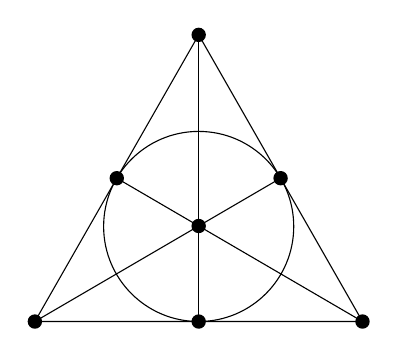
\begin{tikzpicture}[scale=1.3]
% 三角形的三个顶点
\coordinate (A) at (0,1.8);
\coordinate (B) at (-1.6,-1);
\coordinate (C) at (1.6,-1);
% 三边中点
\coordinate (MBC) at (0,-1);
\coordinate (MCA) at (0.8,0.4);
\coordinate (MAB) at (-0.8,0.4);
% 重心
\coordinate (Gc) at (0,-0.0667);
\draw (A)--(B)--(C)--(A);
\draw (A)--(MBC);
\draw (B)--(MCA);
\draw (C)--(MAB);
\draw (0,-0.0714) circle (0.9286);
\fill (A) circle (2pt); \fill (B) circle (2pt); \fill (C) circle (2pt);
\fill (MBC) circle (2pt); \fill (MCA) circle (2pt); \fill (MAB) circle (2pt);
\fill (Gc) circle (2pt);
\end{tikzpicture}

图 1
\end{center}

这个平面的\textbf{自同构}是保持关联关系的点与直线的一个置换。例如图 1 中三角形的六个对称都给出 \(\mathcal{F}\) 的自同构，但我们将看到 \(\mathcal{F}\) 的自同构比这些多得多。

每个 \(g \in G\) 通过共轭作用在点和直线集合上，且这个作用保持关联关系。只有单位元固定所有点，故通过这个作用，群 \(G\) 将同构于自同构群 \(\operatorname{Aut}(\mathcal{F})\) 的一个子群，\(\operatorname{Aut}(\mathcal{F})\) 是 \(\mathcal{F}\) 的所有自同构构成的群。

容易看出，\(\mathcal{F}\) 的任何固定一条直线上两个点以及不在该直线上的第三个点的自同构固定所有点。因此 \(\mathcal{F}\) 的任何自同构由它在任意三个不共线点上的作用唯一确定。由于容易算出这样的三元组有 168 个，\(\mathcal{F}\) 至多有 168 个自同构。这证明若单群 \(G\) 存在则它唯一，且 \(G \leq \operatorname{Aut}(\mathcal{F})\).

分类过程中还剩下两步：证明 \(\mathcal{F}\) 确实有 168 个自同构，并证明 \(\operatorname{Aut}(\mathcal{F})\) 确实是单群。虽然可以用图论方法做这些，我们采用一个遵循“代数群”理论思想的方法。设 \(V\) 是 2 元域 \(\mathbb{F}_2\) 上的 3 维向量空间，故 \(V\) 是 8 阶初等阿贝尔 2-群 \(Z_2 \times Z_2 \times Z_2\). 由第 4.4 节命题 17，\(\operatorname{Aut}(V) = GL(V) \cong GL_3(\mathbb{F}_2)\) 的阶为 168. 称 \(V\) 的七个 1 维子空间（即非平凡循环子群）为\textbf{点}，称七个 2 维子空间（即 4 阶子群）为\textbf{直线}，并称点 \(p\) 关联于直线 \(L\)，若 \(p \leq L\). 则容易看出这些点和直线满足与上面相同的公理（11）至（13），因而表示法诺平面。由于 \(GL(V)\) 在这些点和直线上保持关联地忠实作用，\(\operatorname{Aut}(\mathcal{F})\) 的阶至少为 168. 鉴于已建立的 \(|\operatorname{Aut}(\mathcal{F})|\) 的上界，这证明
\[
\operatorname{Aut}(\mathcal{F}) \cong GL(V) \cong GL_3(\mathbb{F}_2)
\]
且 \(\operatorname{Aut}(\mathcal{F})\) 的阶为 168.

最后我们证明 \(GL(V)\) 是单群。反设 \(H\) 是 \(GL(V)\) 的非平凡真正规子群。设 \(Q\) 是这 7 个点组成的集合，\(N\) 是 \(GL(V)\) 中 \(Q\) 的某个点的稳定子。由于 \(GL(V)\) 传递地作用在 \(Q\) 上，\(N\) 的指数为 7. 由于所有 \(N\) 的共轭之交固定所有点，这个交是单位元。于是 \(H \nsubseteq N\)，故 \(GL(V) = HN\). 由于 \(|H : H \cap N| = |HN : N|\)，我们有 \(7 \mid |H|\). 由于 \(GL(V)\) 同构于 \(S_7\) 的子群，且 \(S_7\) 的西罗 7-子群的正规化子阶为 42，\(GL(V)\) 没有正规的西罗 7-子群，故由西罗定理 \(n_7(GL(V)) = 8\). \(H\) 的正规西罗 7-子群将在 \(H\) 中特征，因而在 \(GL(V)\) 中正规，故 \(H\) 也没有唯一的西罗 7-子群。由于 \(n_7(H) \equiv 1 \pmod 7\) 且 \(n_7(H) \leq n_7(GL(V)) = 8\)，必有 \(n_7(H) = 8\). 这意味着 \(|H|\) 被 8 整除，故 \(56 \mid |H|\)，且由于 \(H\) 真，必有 \(|H| = 56\). 由通常的计数论证（参见第 5.5 节习题 7(b)）\(H\) 有正规的、因而特征的西罗 2-子群，它在 \(GL(V)\) 中正规。但这样 \(GL(V)\) 将有唯一的西罗 2-子群。由于上三角矩阵的集合和下三角矩阵的集合是 \(GL_3(\mathbb{F}_2)\) 的两个各含 8 个元素的子群，我们得到矛盾。总之我们现在证明了下面的定理。

\begin{theorem}\label{thm:6.15}
在同构意义下，168 阶单群唯一，即 \(GL_3(\mathbb{F}_2)\)，它也是射影平面 \(\mathcal{F}\) 的自同构群。
\end{theorem}

注意我们完全可以称 \(W_j\) 为点、\(U_i\) 为直线。点与直线之间的这种“对偶性”连同 168 阶单群的唯一性，可以用来证明 \(G\) 有一个交换点和直线的外自同构，即把 \(U\) 共轭为 \(W\).

许多族有限单群可以用类似的方法分类。在更一般的框架中，称为\textbf{建筑}的几何结构扮演射影平面的角色（射影平面是 \(A_2\) 型建筑的特例）。在这种背景下，子群 \(N_G(U)\) 和 \(N_G(W)\) 是 \(G\) 的\textbf{抛物子群}，\(U, W\) 分别是它们的\textbf{幂幺根}。特别地，所有单线性群（参见 3.4 节）都由其抛物子群的结构与交、等价地由它们在某个相伴建筑上的作用来刻画。

\subsection*{关于群的存在性问题的注记}

如同数学的其他领域（例如微分方程理论），人们可以假设某个数学系统（例如某个方程的解）存在，并由此推出关于这个假设系统的大量信息。一般地，若在相当的努力之后仍未基于初始假设得到矛盾，人们就开始怀疑确实存在满足所假设条件的系统。然而，再多的自洽数据也不能证明存在性。假设我们对一个假想的 \(3^3 \cdot 7 \cdot 13 \cdot 409\) 阶单群 \(G\) 做类似于我们对 168 阶单群（我们证明了它存在）所做的分析。经过一定努力后我们可以证明可能的西罗数唯一：
\[
n_3 = 7 \cdot 409, \quad n_{13} = 3^2 \cdot 7 \cdot 409, \quad n_{409} = 3^2 \cdot 7 \cdot 13.
\]
我们还可以进一步证明这样的 \(G\) 不含 \(pq\) 阶元素（\(p, q\) 是不同素数）、不含 9 阶元素，且不同的西罗子群交为单位元。然后我们可以对所有素数 \(p\) 计数西罗 \(p\)-子群中的元素，会发现总数恰好等于 \(|G|\). 此时我们就有了 \(G\) 的完整子群结构和类方程。我们可能猜测存在这个阶的单群，但费特—汤普森定理断言不存在奇数合数阶的单群。（不过要注意，可能的 \(3^3 \cdot 7 \cdot 13 \cdot 409\) 阶单群的构型属于费特—汤普森定理证明中必须处理的情形之一，故在这种情况下引用这个结果实际上是循环论证。我们在 19.3 节证明不存在这个阶的单群；另见习题 29。）要点是：即使在这种情况下我们拥有的数据与 168 阶情形一样多（即命题 \ref{pro:6.14}），没有某种新技巧我们也无法证明存在性。

当我们处理非单群时，至少有从较小群构造较大群的方法：半直积。尽管这个方法相当受限，它传达了一个观念：非单群可以以某种构造方式由较小群搭建起来。这个过程对单群完全失效；因此技巧的这种分界加强了我们对赫尔德纲领的理解：确定单群，并找出这些群如何拼在一起形成更大的群。

对单群的研究，如上面的 168 阶群讨论所示，使用与非单群研究相同的许多工具（以揭示其子群结构等），但也需要其他构造技巧。正如我们在那番讨论末尾提到的，这些技巧往往涉及代数或几何方法，把单群构造成具有内在趣味的数学结构的自同构，从而以引人入胜的方式把群论与数学和科学的其他领域联系起来。因此虽然我们在有限群的分析上已经走了很远，这个分支中还有许多不同的领域我们只是刚刚触及。

对无限群的分析一般涉及相当不同的方法，下一节我们介绍其中一些。

\subsection*{习题}

\noindent\textbf{计算元素：}

\begin{enumerate}
\item 证明对固定的 \(P \in \operatorname{Syl}_p(G)\)，若对所有 \(R \in \operatorname{Syl}_p(G) - \{P\}\) 有 \(P \cap R = 1\)，则只要 \(P_1, P_2\) 是 \(G\) 的不同西罗 \(p\)-子群就有 \(P_1 \cap P_2 = 1\). 由此推出此时 \(G\) 中 \(p\)-幂阶非单位元的个数是 \((|P| - 1)|G : N_G(P)|\).

\item 在群 \(S_3 \times S_3\) 中举出一对交为单位元的西罗 2-子群，并举出另一对交为 2 阶群的西罗 2-子群。

\item 证明若 \(|G| = 380\)，则 \(G\) 不单。〔只需计数奇数素数阶元素。〕

\item 证明不存在 80、351、3875 或 5313 阶单群。

\item 设 \(G\) 是可解群，阶为 \(pm\)，其中 \(p\) 是不整除 \(m\) 的素数，\(P \in \operatorname{Syl}_p(G)\). 若 \(N_G(P) = P\)，证明 \(G\) 有 \(m\) 阶正规子群。证明中哪里用到了 \(G\) 的可解性？（这个结果对非可解群也成立——它是伯恩赛德 \(N/C\) 定理的特例。）
\end{enumerate}

\noindent\textbf{利用小指数子群：}

\begin{enumerate}\setcounter{enumi}{5}
\item 证明不存在 2205、4125、5103、6545 或 6435 阶单群。
\end{enumerate}

\noindent\textbf{置换表示：}

\begin{enumerate}\setcounter{enumi}{6}
\item 证明不存在 1755 或 5265 阶单群。〔用西罗 3-子群证明 \(G \leq S_{13}\)，并考察西罗 13-子群的正规化子。〕

\item 证明不存在 792 或 918 阶单群。

\item 证明不存在 336 阶单群。
\end{enumerate}

\noindent\textbf{让 \(p\)-子群相互制约：}

\begin{enumerate}\setcounter{enumi}{9}
\item 证明不存在 4095、4389、5313 或 6669 阶单群。

\item 证明不存在 4851 或 5145 阶单群。

\item 证明不存在 9555 阶单群。〔设 \(Q \in \operatorname{Syl}_{13}(G)\)，\(P \in \operatorname{Syl}_7(N_G(Q))\). 论证 \(Q \trianglelefteq N_G(P)\)——为什么这是矛盾？〕
\end{enumerate}

\noindent\textbf{西罗交的正规化子：}

\begin{enumerate}\setcounter{enumi}{12}
\item 设 \(G\) 有不止一个西罗 \(p\)-子群。在所有不同西罗 \(p\)-子群对中取 \(P, Q\) 使 \(|P \cap Q|\) 最大。证明 \(N_G(P \cap Q)\) 有不止一个西罗 \(p\)-子群，且 \(N_G(P \cap Q)\) 的任意两个不同西罗 \(p\)-子群交为子群 \(P \cap Q\).（于是 \(|N_G(P \cap Q)|\) 被 \(p \cdot |P \cap Q|\) 整除，也被某个非 \(p\) 的素数整除。注意 \(N_G(P \cap Q)\) 的西罗 \(p\)-子群不必是 \(G\) 的西罗子群。）

\item 证明不存在 144、525、2025 或 3159 阶单群。
\end{enumerate}

\noindent\textbf{综合习题：}

\begin{enumerate}\setcounter{enumi}{14}
\item 分类 105 阶群。

\item 证明不存在小于 10000 的奇数阶非阿贝尔单群。

\item （a）证明不存在 420 阶单群。

（b）证明不存在小于 500 的偶数阶单群，除了阶为 2, 60, 168, 360 的情形。

\item 证明：若 \(G\) 是 36 阶群，则 \(G\) 有正规的西罗 2-子群或正规的西罗 3-子群。

\item 证明没有 6 阶子群的 12 阶群同构于 \(A_4\).

\item 证明没有 6 阶元素的 24 阶群同构于 \(S_4\).

\item 把引理 \ref{lem:6.13} 推广如下：证明若 \(n_p \not\equiv 1 \pmod{p^k}\)，则存在 \(G\) 的不同西罗 \(p\)-子群 \(P, R\)，使 \(P \cap R\) 在 \(P\) 和 \(R\) 中的指数都不超过 \(p^{k-1}\).

\item 假设在 \(G\) 的所有不同西罗 \(p\)-子群对中取 \(P, R\) 使 \(|P \cap R|\) 最大。证明 \(N_G(P \cap R)\) 不是 \(p\)-群。

\item 设 \(A\) 和 \(B\) 是 \(G\) 的西罗 \(p\)-子群 \(P\) 的正规子集。证明若 \(A\) 和 \(B\) 在 \(G\) 中共轭，则它们在 \(N_G(P)\) 中共轭。

\item 设 \(G\) 是 \(pqr\) 阶群，\(p, q, r\) 是素数且 \(p < q < r\). 证明 \(G\) 的西罗 \(r\)-子群正规。

\item 设 \(G\) 是 \(p^2qr\) 阶单群，其中 \(p, q, r\) 是素数。证明 \(|G| = 60\).

\item 证明或举反例否定如下断言：若 \(G\) 是 168 阶群且有不止一个西罗 7-子群，则 \(G\) 是单群。

\item 证明：若 \(\mathcal{F}\) 是满足 168 阶单群小节中性质（11）至（13）的任意点和直线集合，则 \(\mathcal{F}\) 的关联图被唯一确定，且与图 1 相同（在点和直线重标号的意义下）。〔取一条直线和不在它上面的任意点。把这条直线画成等边三角形的底边，把这个点画成不在底边上的顶点。用公理证明其余点和直线的关联随后被唯一确定，如图 1 所示。〕

\item 设 \(G\) 是 \(3^3 \cdot 7 \cdot 13 \cdot 409\) 阶单群。对每个 \(p \in \{3, 7, 13, 409\}\) 计算 \(n_p\) 的所有允许取值，并化归到每个 \(n_p\) 只有一个可能值的情形。

\item 已知假想的 \(3^3 \cdot 7 \cdot 13 \cdot 409\) 阶单群的西罗数信息，证明不存在这样的群。〔用 819 次的置换表示。〕

\item 假设 \(G\) 是 720 阶单群。尽可能多地求出 \(G\) 的性质（西罗数、西罗子群的同构类型、共轭类等）。这样的群存在吗？
\end{enumerate}

\section{关于自由群的几句话}

本节我们介绍所谓\textbf{自由群}的基本理论。这将使我们能精确表述前面各章中使用的生成元和关系的概念。本节的结果只依赖于同态的基本理论。

由集合 \(S\) 生成的自由群 \(F(S)\) 的基本想法是：\(S\) 中任何元素都不满足任何关系（\(S\) 是“无关系”的）。例如，若 \(S\) 是集合 \(\{a, b\}\)，则两个生成元 \(a\) 和 \(b\) 上的自由群的元素形如 \(a, aa, ab, abab, bab\) 等，称为 \(a\) 和 \(b\) 中的\textbf{词}，连同这些元素的逆元，且所有这些元素都视为不同的。若把同类项合并，我们就得到熟悉形式的元素 \(a, b^{-3}, aba^{-1}b^2\) 等。这样的元素通过把它们的词连接起来相乘（例如 \(aba\) 与 \(b^{-1}a^3b\) 的乘积就是 \(aba\,b^{-1}a^3b\)）。一开始（甚至在我们知道 \(S\) 包含在某个群中之前）自然地把 \(F(S)\) 简单地定义为 \(S\) 中所有词的集合，其中两个这样的表达式在 \(F(S)\) 中通过连接它们相乘。虽然本质上这就是我们要做的，但为了证明这个连接运算是良定义的、结合的，需要更形式化一些。毕竟，连乘积 \(a \cdot a \cdots a\)（\(n\) 项）的熟悉记号 \(a^n\) 之所以允许，也只是因为我们已经知道这个乘积与括号方式无关（参见 1.1 节广义结合律）。\(F(S)\) 的形式化构造在下面就任意集合 \(S\) 进行。

反映 \(S\) 中生成元不必满足任何关系这一事实的一个重要性质是：从集合 \(S\) 到群 \(G\) 的任何映射都可以唯一地延拓为从群 \(F(S)\) 到 \(G\) 的同态（基本上是因为我们已经指定了生成元必须映到哪里，而所有其他元素的像由同态性质唯一确定——没有关系需要担心这一事实意味着我们可以任意指定生成元的像）。这常称为自由群的\textbf{泛性质}，事实上它刻画了群 \(F(S)\).

“自由性”这一概念出现在许多代数系统中，可能已经从初等向量空间理论（用不同的术语）中熟悉。当代数系统是向量空间时，\(F(S)\) 就是以 \(S\) 为基的向量空间。这个空间中的每个向量都是 \(S\) 中元素的唯一线性组合（“词”的类比）。从基 \(S\) 到另一个向量空间 \(V\) 的任何集合映射都唯一地延拓为从 \(F(S)\) 到 \(V\) 的线性变换（即向量空间同态）。

在开始构造 \(F(S)\) 之前，我们提到人们常用交换图的语言描述泛性质。这种形式（对群）如下：给定从集合 \(S\) 到群 \(G\) 的任何集合映射 \(\varphi\)，存在唯一的同态 \(\Phi : F(S) \to G\) 使 \(\Phi|_S = \varphi\)，即下图交换：

\begin{center}
\begin{tikzpicture}[scale=1.1]
\node (S) at (0,2) {$S$};
\node (F) at (3.2,2) {$F(S)$};
\node (G) at (1.6,0) {$G$};
\draw[->] (S)--node[above]{包含映射}(F);
\draw[->] (S)--node[left]{$\varphi$}(G);
\draw[->,dashed] (F)--node[right]{$\Phi$}(G);
\end{tikzpicture}
\end{center}

如上所述，构造 \(F(S)\) 的唯一困难在于验证 \(F(S)\) 中词的连接运算是良定义的、结合的。为证明词乘法的结合性，我们回到最基本的层次，即 \(S\) 的词中所有指数都是 \(\pm 1\).

我们首先为 \(S\) 的元素引入逆元和单位元。设 \(S^{-1}\) 是与 \(S\) 不交的任意集合，使得存在从 \(S\) 到 \(S^{-1}\) 的双射。对每个 \(s \in S\) 用 \(s^{-1}\) 表示它在 \(S^{-1}\) 中对应的元素；类似地，对每个 \(t \in S^{-1}\) 把 \(S\) 中对应的元素记为 \(t^{-1}\)（故 \((s^{-1})^{-1} = s\)）。取一个不在 \(S \cup S^{-1}\) 中的单元素集，称之为 \(\{1\}\). 令 \(1^{-1} = 1\)，并对任意 \(x \in S \cup S^{-1} \cup \{1\}\) 令 \(x^1 = x\).

下面我们描述集合 \(S\) 上自由群的元素。\(S\) 上的\textbf{词}按定义是序列
\[
(s_1, s_2, s_3, \ldots), \quad \text{其中 } s_i \in S \cup S^{-1} \cup \{1\},
\]
且对所有充分大的 \(i\) 有 \(s_i = 1\)（即对每个序列存在 \(N\) 使对所有 \(i \geq N\) 有 \(s_i = 1\)）。因此我们可以把一个词看作 \(S\) 的元素及其逆元的有限乘积（允许重复）。接下来，为保证表达式的唯一性，我们只考虑在相邻项之间没有明显“消去”的词（如 \(baa^{-1}b = bb\)）。词 \((s_1, s_2, s_3, \ldots)\) 称为\textbf{既约的}，若

（1）对所有满足 \(s_i \neq 1\) 的 \(i\) 有 \(s_{i+1} \neq s_i^{-1}\)，且

（2）若对某个 \(k\) 有 \(s_k = 1\)，则对所有 \(i \geq k\) 有 \(s_i = 1\).

既约词 \((1, 1, 1, \ldots)\) 称为\textbf{空词}，记作 \(1\). 我们现在通过把既约词 \((s_1^{\epsilon_1}, s_2^{\epsilon_2}, \ldots, s_n^{\epsilon_n}, 1, 1, 1, \ldots)\)（\(s_i \in S\)，\(\epsilon_i = \pm 1\)）写成 \(s_1^{\epsilon_1}s_2^{\epsilon_2}\cdots s_n^{\epsilon_n}\) 来简化记号。注意按定义，既约词 \(r_1^{\delta_1}r_2^{\delta_2}\cdots r_m^{\delta_m}\) 与 \(s_1^{\epsilon_1}s_2^{\epsilon_2}\cdots s_n^{\epsilon_n}\) 相等当且仅当 \(n = m\) 且 \(r_i = s_i\)、\(\delta_i = \epsilon_i\)（\(1 \leq i \leq n\)）。设 \(F(S)\) 是 \(S\) 上既约词的集合，并通过
\[
s \mapsto (s, 1, 1, 1, \ldots)
\]
把 \(S\) 嵌入 \(F(S)\). 在这个集合单射下我们把 \(S\) 与它的像等同，今后把 \(S\) 看作 \(F(S)\) 的子集。注意若 \(S = \varnothing\)，则 \(F(S) = \{1\}\).

现在我们可以引入 \(F(S)\) 上的二元运算。主要的技术困难是保证两个既约词的乘积仍是既约词。虽然定义看起来复杂，它实际上只是“逐次消去”互为逆元的相邻项的形式规则（例如 \(ab^{-1}a\) 乘 \(a^{-1}ba\) 应约化为 \(aa\)）。设 \(r_1^{\delta_1}\cdots r_m^{\delta_m}\) 与 \(s_1^{\epsilon_1}\cdots s_n^{\epsilon_n}\) 是既约词，首先假设 \(m \leq n\). 设 \(k\) 是范围 \(1 \leq k \leq m+1\) 中使 \(s_k^{\epsilon_k} \neq r_{m+1-k}^{-\delta_{m+1-k}}\) 的最小整数。则这两个既约词的乘积定义为
\[
r_1^{\delta_1}\cdots r_m^{\delta_m}\, s_1^{\epsilon_1}\cdots s_n^{\epsilon_n} =
\begin{cases}
r_1^{\delta_1}\cdots r_{m-k+1}^{\delta_{m-k+1}}\, s_k^{\epsilon_k}\cdots s_n^{\epsilon_n}, & \text{若 } k \leq m, \\[2pt]
s_{m+1}^{\epsilon_{m+1}}\cdots s_n^{\epsilon_n}, & \text{若 } k = m+1 \leq n, \\[2pt]
1, & \text{若 } k = m+1 \text{ 且 } m = n.
\end{cases}
\]
当 \(m \geq n\) 时乘积类似地定义，故在两种情形都得到既约词。

\begin{theorem}\label{thm:6.16}
\(F(S)\) 在上述二元运算下是群。
\end{theorem}

\begin{proof}
容易验证 \(1\) 是单位元，且既约词 \(s_1^{\epsilon_1}s_2^{\epsilon_2}\cdots s_n^{\epsilon_n}\) 的逆元是既约词 \(s_n^{-\epsilon_n}s_{n-1}^{-\epsilon_{n-1}}\cdots s_1^{-\epsilon_1}\). 证明的困难部分是验证结合律。这可以通过对所涉及词的“长度”作归纳并考察各种情形来做，也可以如下进行：对每个 \(s \in S \cup S^{-1} \cup \{1\}\)，定义 \(\sigma_s : F(S) \to F(S)\) 为左乘 \(s\)（即把 \(s\) 连到词的左端后的既约化结果）。由于 \(\sigma_s \circ \sigma_{s^{-1}}\) 是 \(F(S) \to F(S)\) 的恒等映射，\(\sigma_s\) 是 \(F(S)\) 的置换。设 \(A(S)\) 是集合 \(F(S)\) 上的对称群中由 \(\{\sigma_s \mid s \in S\}\) 生成的子群。容易看出映射
\[
s_1^{\epsilon_1}s_2^{\epsilon_2}\cdots s_n^{\epsilon_n} \mapsto \sigma_{s_1}^{\epsilon_1} \circ \sigma_{s_2}^{\epsilon_2} \circ \cdots \circ \sigma_{s_n}^{\epsilon_n}
\]
是 \(F(S)\) 与 \(A(S)\) 之间保持二元运算的（集合）双射。由于 \(A(S)\) 是群、因而结合，\(F(S)\) 也结合。
\end{proof}

自由群的泛性质现在容易推出。

\begin{theorem}\label{thm:6.17}
设 \(G\) 是群，\(S\) 是集合，\(\varphi : S \to G\) 是集合映射。则存在唯一的群同态 \(\Phi : F(S) \to G\) 使下图交换：
\begin{center}
\begin{tikzpicture}[scale=1.1]
\node (S) at (0,2) {$S$};
\node (F) at (3.2,2) {$F(S)$};
\node (G) at (1.6,0) {$G$};
\draw[->] (S)--node[above]{包含映射}(F);
\draw[->] (S)--node[left]{$\varphi$}(G);
\draw[->,dashed] (F)--node[right]{$\Phi$}(G);
\end{tikzpicture}
\end{center}
\end{theorem}

\begin{proof}
若 \(\Phi\) 是同态，则它必须满足
\[
\Phi(s_1^{\epsilon_1}s_2^{\epsilon_2}\cdots s_n^{\epsilon_n}) = \varphi(s_1)^{\epsilon_1}\varphi(s_2)^{\epsilon_2}\cdots\varphi(s_n)^{\epsilon_n},
\]
这证明了唯一性；而容易验证这个映射确实是同态，这证明了存在性。
\end{proof}

\begin{corollary}\label{cor:6.18}
\(F(S)\) 在唯一同构的意义下唯一，且这个同构是集合 \(S\) 上的恒等映射。
\end{corollary}

\begin{proof}
这由泛性质推出。假设 \(F(S)\) 和 \(F'(S)\) 是由 \(S\) 生成的两个自由群。由于 \(S\) 同时含于 \(F(S)\) 和 \(F'(S)\) 中，我们有自然的单射 \(S \to F'(S)\) 和 \(S \to F(S)\). 由定理中的泛性质推出有唯一的同态 \(\Phi : F(S) \to F'(S)\) 和 \(\Phi' : F'(S) \to F(S)\)，它们在 \(S\) 上都是恒等映射。复合 \(\Phi'\Phi\) 是从 \(F(S)\) 到 \(F(S)\) 的、在 \(S\) 上为恒等的同态，故由定理中的唯一性陈述，它必是恒等映射。类似地 \(\Phi\Phi'\) 是恒等映射，故 \(\Phi\) 是同构（以 \(\Phi'\) 为逆），证得推论。
\end{proof}

\begin{definition}
群 \(F(S)\) 称为\textbf{集合 \(S\) 上的自由群}。群 \(F\) 称为\textbf{自由群}，若存在集合 \(S\) 使 \(F = F(S)\)——此时我们称 \(S\) 为 \(F\) 的一组\textbf{自由生成元}（或\textbf{自由基}）。\(S\) 的基数称为自由群的\textbf{秩}。
\end{definition}

现在可以用指数记号简化自由群中的表达式，所以我们写 \(a^3b^{-2}\) 而不用形式既约词 \(aaab^{-1}b^{-1}\). 然而像 \(aba\) 这样的表达式在 \(\{a, b\}\) 上的自由群中不能化简。我们提到这个领域的一个重要定理。

\begin{theorem}[施赖埃尔]\label{thm:6.19}
自由群的子群是自由的。
\end{theorem}

这个证明并不平凡，我们不给出证明。这个结果有一个很好的用覆叠空间的证明（参见 J.-P. Serre, Trees, Springer-Verlag, 1980）。

\subsection*{表示}

设 \(G\) 是任意群。则 \(G\) 是自由群的同态像：取 \(S = G\)，\(\varphi\) 为从 \(G\) 到 \(G\) 的恒等映射；则定理 \ref{thm:6.16} 产生一个从 \(F(G)\) 到 \(G\) 的（满）同态。更一般地，若 \(S\) 是 \(G\) 的满足 \(G = \langle S \rangle\) 的任意子集，则同样存在唯一的从 \(F(S)\) 到 \(G\) 的满同态，它在 \(S\) 上是恒等映射。（注意我们现在可以独立地表述子集生成群这一概念：\(G = \langle S \rangle\) 当且仅当延拓 \(S\) 上恒等映射的映射 \(\pi : F(S) \to G\) 是满射。）

\begin{definition}
设 \(S\) 是群 \(G\) 的满足 \(G = \langle S \rangle\) 的子集。\(G\) 的一个\textbf{表示}是一对 \((S, R)\)，其中 \(R\) 是 \(F(S)\) 中词的集合，使得

（1）\(\langle R \rangle\) 在 \(F(S)\) 中的正规闭包（含 \(R\) 的最小正规子群）等于同态 \(\pi : F(S) \to G\) 的核（其中 \(\pi\) 延拓从 \(S\) 到 \(S\) 的恒等映射）。\(\pi(S)\) 的元素称为 \(G\) 的\textbf{生成元}，\(R\) 的元素称为 \(G\) 的\textbf{关系}。

（2）若存在表示 \((S, R)\) 使 \(S\) 是有限集，我们说 \(G\) \textbf{有限生成}；若存在表示 \((S, R)\) 使 \(S\) 和 \(R\) 都是有限集，我们说 \(G\) \textbf{有限表示}。
\end{definition}

注意若 \((S, R)\) 是表示，则映射 \(F(S) \to G\) 的核不是 \(\langle R \rangle\) 本身，而是由 \(R\) 以及 \(R\) 中元素的所有共轭生成的（大得多的）群。注意即使对固定的集合 \(S\)，一个群也会有许多不同的表示（例如我们总可以把冗余关系扔进 \(R\)）。若 \(G\) 有限表示，\(S = \{s_1, s_2, \ldots, s_n\}\)，\(R = \{w_1, w_2, \ldots, w_k\}\)，我们写（如前面各章所做）：
\[
G = \langle s_1, s_2, \ldots, s_n \mid w_1 = w_2 = \cdots = w_k = 1 \rangle,
\]
而若 \(w\) 是词 \(w_1w_2^{-1}\)，我们就写 \(w_1 = w_2\) 而不是 \(w = 1\).

\begin{example}
（1）每个有限群都有限表示。为看出这一点，设 \(G = \{g_1, \ldots, g_n\}\) 是有限群。令 \(S = G\)，\(\pi : F(S) \to G\) 是延拓 \(S\) 上恒等映射的同态。设 \(R_0\) 是词 \(g_ig_jg_k^{-1}\) 的集合，其中 \(i, j = 1, \ldots, n\) 且 \(g_ig_j = g_k\)（在 \(G\) 中）。显然 \(R_0 \leq \ker \pi\). 若 \(N\) 是 \(R_0\) 在 \(F(S)\) 中的正规闭包，\(\bar{G} = F(S)/N\)，则 \(\bar{G}\) 是 \(G\) 的同态像（即 \(\pi\) 通过 \(N\) 分解）。此外，元素集合 \(\{\bar{g}_i \mid i = 1, \ldots, n\}\) 对乘法封闭。由于这个集合生成 \(\bar{G}\)，它必等于 \(\bar{G}\). 于是 \(|\bar{G}| = |G|\)，故 \(N = \ker \pi\)，\((S, R_0)\) 是 \(G\) 的一个表示。

这说明了 \((S, R)\) 是给定有限群 \(G\) 的表示的一个充分条件：

（i）\(S\) 必须是 \(G\) 的生成集，且

（ii）任何由 \(S\) 生成、满足 \(R\) 中关系的群，其阶必不超过 \(|G|\).

（2）阿贝尔群容易表示。例如
\[
\mathbb{Z} \cong F(\{a\}) = \langle a \rangle, \qquad \mathbb{Z} \times \mathbb{Z} \cong \langle a, b \mid [a, b] = 1 \rangle,
\]
\[
Z_n \times Z_m \cong \langle a, b \mid a^n = b^m = [a, b] = 1 \rangle.
\]
（回忆 \([a, b] = a^{-1}b^{-1}ab\)。）

（3）前面各章引入的一些熟悉的非阿贝尔群有简单的表示：
\[
D_{2n} = \langle r, s \mid r^n = s^2 = 1,\ s^{-1}rs = r^{-1} \rangle,
\]
\[
Q_8 = \langle i, j \mid i^4 = 1,\ j^2 = i^2,\ j^{-1}ij = i^{-1} \rangle.
\]
为检验例如 \(D_{2n}\) 的表示，注意表示 \(\langle r, s \mid r^n = s^2 = 1,\ s^{-1}rs = r^{-1} \rangle\) 中的关系蕴含这个群有一个（由 \(r\) 生成的）阶不超过 \(n\) 的正规子群，其商由 \(s\) 生成（\(s\) 的阶不超过 2）。于是任何具有这些生成元和关系的群阶至多为 \(2n\). 由于我们已经知道存在满足这些条件的 \(2n\) 阶群 \(D_{2n}\)，这个抽象表示必等于 \(D_{2n}\).

（4）如 1.2 节所述，一般地，即使判定给定的一组生成元和关系是否给出平凡群都是极其困难的（更不用说判定它是否是某个其他非平凡有限群了）。例如在下面两个表示中，第一个群是无限群，第二个是平凡群（参见 Trees, 第 1 章）：
\[
\langle x_1, x_2, x_3, x_4 \mid x_2x_1x_2^{-1} = x_1^2,\ x_3x_2x_3^{-1} = x_2^2,\ x_4x_3x_4^{-1} = x_3^2,\ x_1x_4x_1^{-1} = x_4^2 \rangle,
\]
\[
\langle x_1, x_2, x_3 \mid x_2x_1x_2^{-1} = x_1^2,\ x_3x_2x_3^{-1} = x_2^2,\ x_1x_3x_1^{-1} = x_3^2 \rangle.
\]

（5）容易看出 \(S_n\) 由对换 \((1\,2), (2\,3), \ldots, (n-1\ n)\) 生成，且它们满足关系
\[
((i\ i+1)(i+1\ i+2))^3 = 1, \qquad [(i\ i+1),\ (j\ j+1)] = 1 \quad (\text{当 } |i-j| \geq 2),
\]
（这里 \(|i-j|\) 表示整数 \(i-j\) 的绝对值）。可以对 \(n\) 作归纳证明这些构成 \(S_n\) 的一个表示：
\[
S_n \cong \langle t_1, \ldots, t_{n-1} \mid t_i^2 = 1,\ (t_it_{i+1})^3 = 1,\ [t_i, t_j] = 1\ (\text{当 } |i-j| \geq 2),\ 1 \leq i, j \leq n-1 \rangle.
\]
\end{example}

如 1.6 节所述，我们可以用群的表示来求群之间的同态或求群的自同构。我们在分类 6 阶群时就是这么做的，例如当我们证明任何 6 阶非阿贝尔群都由一个 3 阶元素和一个把它取逆的 2 阶元素生成时：于是存在从 \(S_3\) 到任何 6 阶非阿贝尔群上的同态（由阶的计算可知它是同构）。更一般地，假设 \(G\) 由生成元（例如）\(a, b\) 和关系 \(r_1, \ldots, r_k\) 表示。若 \(a', b'\) 是群 \(H\) 的任意元素，满足这些关系，则存在从 \(G\) 到 \(H\) 的同态。也就是说，若 \(\pi : F(\{a, b\}) \to G\) 是表示同态，我们可以通过 \(\pi'(a) = a'\)、\(\pi'(b) = b'\) 定义 \(\pi' : F(\{a, b\}) \to H\). 则 \(\ker \pi \leq \ker \pi'\)，故 \(\pi'\) 通过 \(\ker \pi\) 分解，得到
\[
G \cong F(\{a, b\})/\ker \pi \to H.
\]
特别地，若 \(\langle a', b' \rangle = H = G\)，这个同态是 \(G\) 的自同构。

反之，任何自同构必把一组生成元送到另一组满足相同关系的生成元。例如 \(D_8 = \langle a, b \mid a^2 = b^4 = 1,\ aba = b^{-1} \rangle\)，任何一对元素 \(a', b'\)（其中 \(a'\) 是 2 阶非中心元素，\(b'\) 是 4 阶元素）满足相同的关系。由于有四个 2 阶非中心元素和两个 4 阶元素，\(D_8\) 有 8 个自同构。

类似地，\(Q_8\) 中任何一对 4 阶元素，只要互不相等也不互为逆元，就必生成 \(Q_8\) 且满足上面例 3 中给出的关系。容易验证这样的元素对有 24 个，故
\[
|\operatorname{Aut}(Q_8)| = 24.
\]

自由对象可以在（许多但并非全部）其他范畴中构造。例如，\textbf{幺半群}是带有一个满足除存在逆元公理之外所有群公理的二元运算的集合。幺半群范畴中的自由对象在理论计算机科学中起基础作用，那里它们为机器（图灵机等）的行为建模。我们将在后面各章遇到自由代数（即多项式代数）和自由模。

\subsection*{习题}

\begin{enumerate}
\item 设 \(F_1\) 和 \(F_2\) 是有限秩自由群。证明 \(F_1 \cong F_2\) 当且仅当它们有相同的秩。要把你的证明推广到无限秩（此时结果也成立），你需要什么事实？

\item 证明：若 \(|S| > 1\)，则 \(F(S)\) 非阿贝尔。

\item 证明 2 个生成元上的自由群的交换子子群不是有限生成的（特别地，有限生成群的子群不必有限生成）。

\item 证明自由群的每个非单位元都是无限阶的。

\item 用 2 个生成元给出 \(A_4\) 的一个有限表示。

\item 用 2 个生成元给出 \(S_4\) 的一个有限表示。

\item 证明下面的是 8 阶四元数群的一个表示：
\[
Q_8 = \langle a, b \mid a^2 = b^2,\ a^{-1}ba = b^{-1} \rangle.
\]

\item 用表示求群 \(Z_2 \times Z_4\) 和 \(Z_4 \times Z_4\) 的自同构群的阶。

\item 证明 \(\operatorname{Aut}(Q_8) \cong S_4\).

\item 这个习题给出 \(S_6\) 的一个非内自同构（因此它连同第 4.4 节习题 19 表明 \(|\operatorname{Aut}(S_6) : \operatorname{Inn}(S_6)| = 2\)）。设
\[
t_1 = (1\,2)(3\,4)(5\,6),\quad t_2 = (1\,4)(2\,5)(3\,6),\quad t_3 = (1\,3)(2\,4)(5\,6),
\]
\[
t_4 = (1\,2)(3\,6)(4\,5),\quad t_5 = (1\,4)(2\,3)(5\,6).
\]
证明 \(t_1, \ldots, t_5\) 满足下列关系：
\[
(t_i)^2 = 1\ (\text{对所有 } i), \quad (t_it_j)^2 = 1\ (\text{对所有 } |i-j| \geq 2), \quad (t_it_{i+1})^3 = 1\ (\text{对所有 } i \in \{1,2,3,4\}).
\]
由此推出 \(S_6 = \langle t_1, \ldots, t_5 \rangle\)，且映射
\[
(1\,2) \mapsto t_1,\quad (2\,3) \mapsto t_2,\quad (3\,4) \mapsto t_3,\quad (4\,5) \mapsto t_4,\quad (5\,6) \mapsto t_5
\]
延拓为 \(S_6\) 的一个自同构（它显然不是内的，因为它不把对换送到对换）。〔使用例 5 中描述的 \(S_6\) 的表示。〕

\item 设 \(S\) 是集合。表示 \((S, R)\)（其中 \(R = \{[s, t] \mid s, t \in S\}\)）的群称为 \(S\) 上的\textbf{自由阿贝尔群}——记作 \(A(S)\). 证明 \(A(S)\) 具有如下泛性质：若 \(G\) 是任意阿贝尔群，\(\varphi : S \to G\) 是任意集合映射，则存在唯一的群同态 \(\Phi : A(S) \to G\) 使 \(\Phi|_S = \varphi\). 由此推出：若 \(A\) 是基数为 \(n\) 的集合上的自由阿贝尔群，则
\[
A \cong \mathbb{Z} \times \mathbb{Z} \times \cdots \times \mathbb{Z} \quad (n \text{ 个因子}).
\]

\item 设 \(S\) 是集合，\(c\) 是正整数。表述 \(S\) 上幂零类为 \(c\) 的\textbf{自由幂零群}的概念，并证明它对幂零类为 \(c\) 的幂零群具有相应的泛性质。

\item 证明不存在由两个元素生成的幂零群 \(N\)，具有性质：每个由两个元素生成的幂零群都是 \(N\) 的同态像（即前一题中幂零类 \(c\) 的指定是必要的）。
\end{enumerate}
